\documentclass[11pt]{article}
\usepackage[T1]{fontenc}
\usepackage[utf8]{inputenc}
\usepackage[margin=1.0in]{geometry}
\usepackage{indentfirst}
\usepackage{changepage}
\usepackage{gensymb}
\usepackage{rotating}
\usepackage{lscape}
\usepackage{pdfpages}
\usepackage{enumitem}
\usepackage{graphicx}
\usepackage{adjustbox}
\usepackage{float}
\usepackage{csvsimple}
\usepackage{authblk}
\usepackage{listings}

\usepackage{hyperref}
\hypersetup{
    colorlinks=true,
    linkcolor=blue,
    filecolor=magenta,      
    urlcolor=cyan,
}
\urlstyle{same}

\newlist{steps}{enumerate}{1}
\setlist[steps, 1]{label = Step \arabic*:}



\title{Acceptance Study for SciBooNE Charged-Current Coherent Pion Production Technical Note Rough Draft}
\author[1]{Jonathan Asaadi\thanks{jonathan.asaadi@uta.edu}}
\author[1]{Zachary Williams\thanks{zachary.williams2@mavs.uta.edu}}
\affil[1]{Department of Physics, The University of Texas at Arlington}

\renewcommand\Authands{ and }

%|------------------------------The Document Begins Here------------------------
\begin{document}

%|------------------------------The Title Page Begins Here---------------------
\begin{minipage}[h]{\textwidth}
\maketitle
\begin{abstract}
We showed that the SciBooNE guys tried to mess physics up by cutting out all of their CC-Coh Pion events from their data that was actually there! Duh.


Do we need an abstract?
\end{abstract}
\end{minipage}
%|===============================The Title Page Ends Here============================



%=====================================================
\section{Introduction}\label{sec:introduction}
%=====================================================
The goal of this document is to provide a reference for the acceptance study performed for the SciBooNE charged current coherent pion re-analysis as well as provide documentation to the code used in this study (in the event anything needs to be revisited in the future).

The code currently lives in this github repository labeled \href{https://github.com/williamszg/SciBooNE-MC}{SciBooNE-MC} and the corresponding ROOT files used in the simulation can be downloaded from here (insert dropbox/Google Drive Link here)

The paper is structured such that Section \ref{sec:samples} outlines samples used in this study, Section \ref{sec:simulation} describes the SciBooNE detector as it was simulated in this study, Section \ref{sec:Results} gives a high level summary of the results including the event-reduction table as well as the CC-Coh-$\pi$ acceptance results.

Sections \ref{} - \ref{} provide supporting plots which are used to generate the acceptance tables found in Section \ref{}. 

The appendix is left to explain how the code is run and the details of the scripts within.

%----------------------------------------
\subsection{Goal}\label{sec:goals}
%----------------------------------------
The goal of the reanalysis is to examine the acceptance modeling for the SciBooNE results in the presence of modern neutrino generators and updated models in order to understand why SciBooNE did not observe Charged-Current Coherent Pion Production at low neutrino energy. The purpose of this acceptance study is to blah blah blah... (coming back to this later...)



%=====================================================
\section{Samples}\label{sec:samples}
%=====================================================
Five different samples were used in this study, three samples for $\nu$-mode and two samples in $\bar{\nu}$-mode.\footnote{All of these samples were generated by Callum Wilkinson (Thanks, Callum!)} Table \ref{tab:samples} summarizes these samples. Details on these samples can be found in Appendix 

\begin{center}
\begin{table}[htb]
	\begin{center}
	%\resizebox{0.45\textwidth}{!}
	\caption{Summary of the samples used to build the acceptance model for this study.} \label{tab:samples}
	\end{center}
\end{table}
\end{center}



%=======================================================================
\section{Simulation}\label{sec:simulation}
%=======================================================================
This section is intended to detail the nuances of this acceptance model, and to detail what assumptions are made in the acceptance modeling to result in accurate classifications of events as Charged-Current Coherent Pion Production.

%-----------------------------------------------------------------------------------------------------------------|
\subsection{The Detector}
For the purposes of this acceptance study, the SciBooNE experiment is composed of two sub-detectors. The first (and the more upstream) of the sub-detectors, is the Scintillator Bar Tracker (SciBar) which was originally conceived and constructed to function as the near detector for the K2K experiment [reference]. The second (and more downstream) of the sub-detectors, is the Muon Range Detector (MRD), which is the detector designed and constructed specifically for SciBooNE for measuring the momentum of muons produced from charged-current neutrino interactions up to $1.2$ $GeV/c$ by using the observed range of the trajectory of the muon. These detectors and the corresponding coordinate system we will use throughout this note are shown in Figure \ref{fig:SciBooNEDetector}

\begin{figure}[H]
\centering
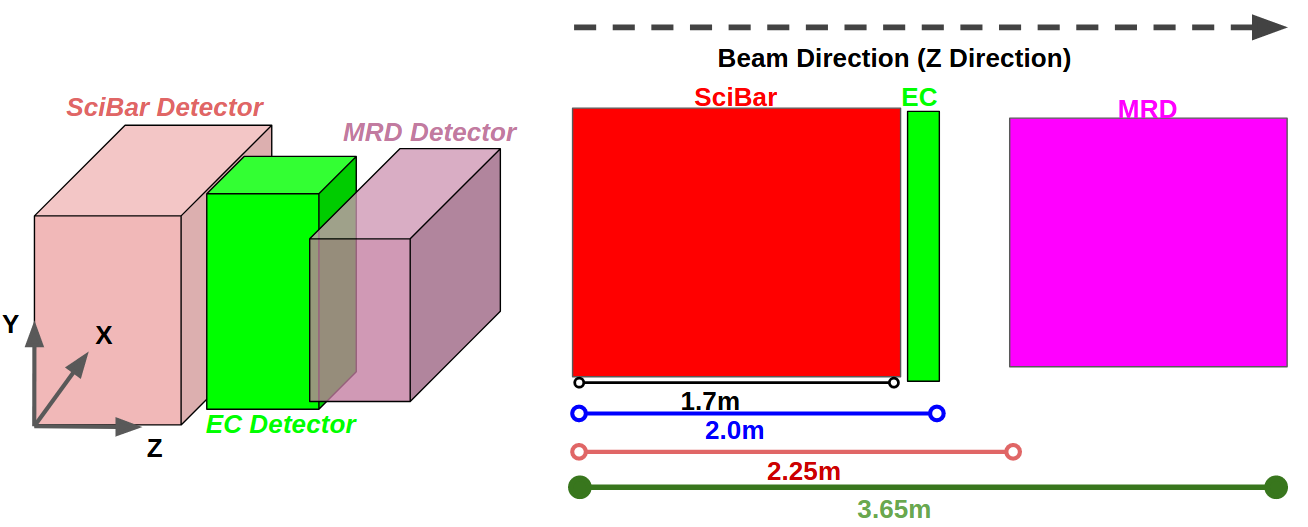
\includegraphics[width=0.75\textwidth]{EventClassifications/SciBooNEDetector.png}
\caption{Representation of the SciBooNE detector and the coordinate frame we use in this study}
\end{figure}\label{fig:SciBooNEDetector}

\subsubsection{The Scintillator Bar Tracker (SciBar)}
The Scintillator Bar Tracker (SciBar) sub-detector is a scintillator detector (go into more detail?). In this acceptance study, the z-direction starts at 0 at the front face of the SciBar sub-detector. The direction of the beam is in the z-direction, which means the xy-plane is perpindicular to the beam. The dimensions of the sub-detector have the x and y dimensions of the same length of $3.0$ $m$. The z dimension is $1.7$ $m$. This simulation models the scintillator materials as having a constant energy depostion ($dE/dx$) value of $2.04$ $MeV/cm$.

\subsubsection{The Muon Range Detector (MRD)}
The Muon Range Detector (MRD), depicted in Figure \ref{fig:mrd} is located $0.55$ $m$ downstream of SciBar in the z-direction, and is a composition of 2 sets of 13 alternating slabs of steel-scintillator layers, where the scintillator layers alternate between being horizontally oriented or vertically oriented, in the xy-plane. The steel layers have a z-direction thickness of $5.08$ $cm$ and the scintillator layers have a z-direction thickness of $0.6$ $cm$. Combining all the layers of the different alternating materials results in 26 scintillator layers that "sandwich" 25 steel layers inbetween and gives a total z-direction dimension of being $1.37 m$. The xy-plane is modeled as a square again (as was the case with SciBar, too) with dimensions in the x-direction and the y-direction of $2.6$ $m$. The energy deposition ($dE/dx$) of the muon for the scintillator layers is again a constant of $2.04$ $MeV/cm$ and the energy deposition for the steel layers are a constant with value $11.43$ $MeV/cm$.

\begin{figure}[H]
\centering
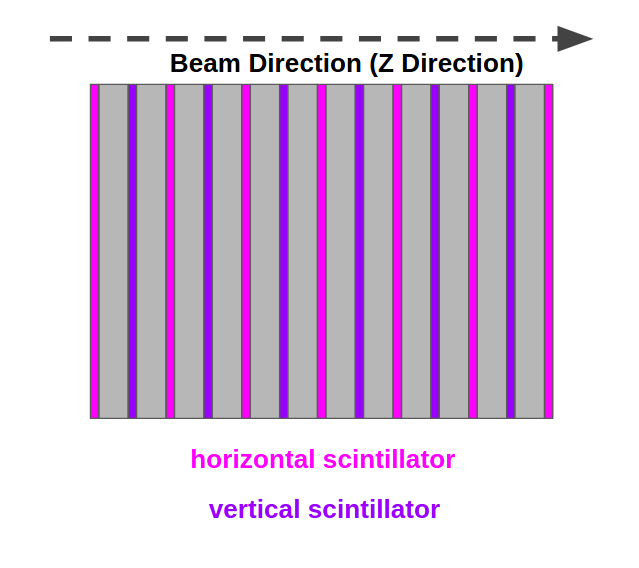
\includegraphics[width=0.75\textwidth]{EventClassifications/mrd.png}
\caption{Depiction of the Muon Range Detector (MRB) which consists of alternating layers of horizontal scintillator (shown in pink) steel slabs (showin in grey) and vertical scintillator (shown in purple)}
\end{figure}\label{fig:mrd}



%=======================================================================
\section{Event Selection}\label{sec:eventselection}
%=======================================================================

%-----------------------------------------------------------------------------------------------------------------|
\subsection{Event Classifications}
There were three different classifications for events that qualified as CC-Coh Pion Production events, that the muon made it to the MRD, and the muon penetrated at least three layers of steel. These categories will be referenced multiple times throughout the remainder of this paper, which makes pertinent that the reader has an understanding of what each of the three specifically mean for any event that falls under any of these classifications.

\subsubsection{Stopped}
An event is classified as "Stopped," if the event qualified as being a CC-Coh Pion Production event, the muon of the event reached the MRD, penetrated three layers of steel, and stopped (or embedded) in the MRD without exiting the sides or the back face. Events that are classified as "Stopped" are included in the combined samples of this acceptance study and are called "Good" events. Maybe put in the dimensions of the xy-plane and z-direction that meet this classification for the MRD? This is shown in the figure below.

\begin{figure}[H]
\centering
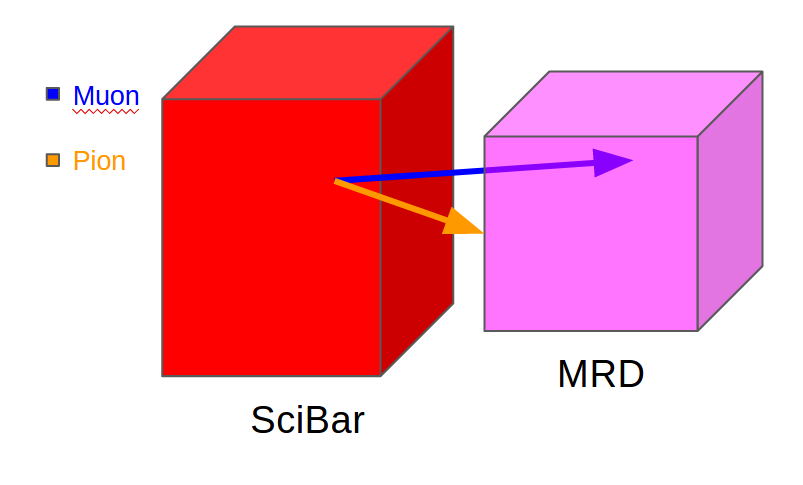
\includegraphics[width=0.6\textwidth]{EventClassifications/Stopped.png}
\caption{Depiction of an event that was classified as "Stopped."}
\end{figure}

\subsubsection{Not-Stopped}
An event is classified as "Not-Stopped," if the event qualified as being a CC-Coh Pion Production event, the muon of the event reached the MRD, and the muon passed out the back face of the MRD without stopping. Events that are classified as "Not-Stopped" are included in the combined samples of this acceptance study and are also called "Good" events. Maybe put in the dimensions of the xy-plane and z-direction that meet this classification for the MRD? This is shown in the figure below.

\begin{figure}[H]
\centering
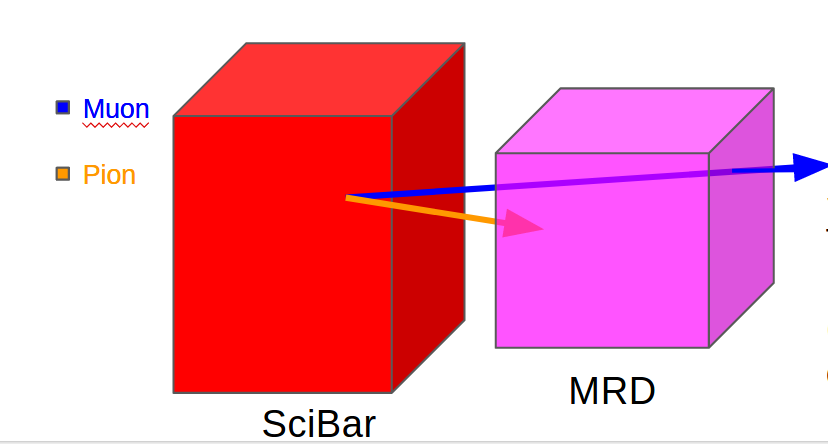
\includegraphics[width=0.6\textwidth]{EventClassifications/NotStopped.png}
\caption{Depiction of an event that was classified as "Not-Stopped."}
\end{figure}

\subsubsection{Out-Side}
An event is classified as "Out-Side," if the event qualified as being a CC-Coh Pion Production event, the muon of the event reached the MRD, penetrated three layers of steel, and then passed through one of the sides of the MRD (not including the back face) without stopping. Events that are classified as "Out-Side" are not included in the combined samples because there was not enough material traversal for an accurate reconstruction of the particles momentum and energy to be made. Maybe put in the dimensions of the xy-plane and z-direction that meet this classification for the MRD? This is shown in the figure below.

\begin{figure}[H]
\centering
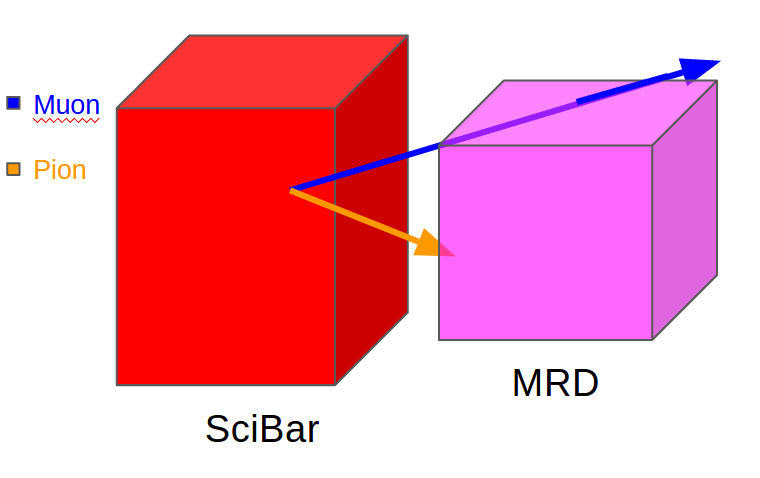
\includegraphics[width=0.6\textwidth]{EventClassifications/OutSide.png}
\caption{Depiction of an event that was classified as "Out-Side."}
\end{figure}

%-----------------------------------------------------------------------------------------------------------------|
\subsection{Stepping Through the Detectors Along an Event}
I do not know if I am really going to include this here or not...
%%%%%%%%%%%%%%%%%%%%%%%%%%% The CC-Coh Pion section ends here! %%%%%%%%%%%%%%%%%%%%%%%%%%%%




%=======================================================================
\section{Results}\label{sec:Results}
%=======================================================================

The results of this acceptance study can be broken down into two different classification schemes of events. Those that met the conditions to qualify as a CC-Inclusive event, and those that met the conditions of classification as Charged-Current Coherent Pion Production events. The plots in the two subsections below show our results.

\subsection{Charged-Current Inclusive Events}\label{sub:CCInclusive}
(You should show the momentum and angle spectrum for the CC-inclusive sample and show that your reproduce the previous efficiency curves)

\subsection{Charged-Current Coherent Pion Production Events}\label{sub:CCCohPion}
(Again, you show the momentum and angle spectrum. You show the 1-d efficiencies and you have the 2-d efficiency plots AND A TABLE WHICH LISTS THEM (this is the biggest piece that is missing and I was expecting to see), here you also include the q2 and |t| distributions and their definitions.)

% Here are the tables for the 2D efficiency histograms
\newpage
\begin{landscape}
\begin{table}
\centering
\caption{Table for 2D Histogram for New NM-Rein-Sehgal}
\begin{adjustbox}{width=\paperwidth}
\csvautotabular{TechNoteTables/New-NM-RS.csv}
\end{adjustbox}
\end{table}
\end{landscape}

\newpage
\begin{landscape}
\begin{table}
\centering
\caption{Table for 2D Histogram for New NM-Berger-Sehgal}
\begin{adjustbox}{width=\paperwidth}
\csvautotabular{TechNoteTables/New-NM-BS.csv}
\end{adjustbox}
\end{table}
\end{landscape}

\newpage
\begin{landscape}
\begin{table}
\centering
\caption{Table for 2D Histogram for Old NM-Rein-Sehgal}
\begin{adjustbox}{width=\paperwidth}
\csvautotabular{TechNoteTables/Old-NM-RS.csv}
\end{adjustbox}
\end{table}
\end{landscape}

\newpage
\begin{landscape}
\begin{table}
\centering
\caption{Table for 2D Histogram for New ANM-Rein-Sehgal}
\begin{adjustbox}{width=\paperwidth}
\csvautotabular{TechNoteTables/New-ANM-RS.csv}
\end{adjustbox}
\end{table}
\end{landscape}

\newpage
\begin{landscape}
\begin{table}
\centering
\caption{Table for 2D Histogram for New ANM-Berger-Sehgal}
\begin{adjustbox}{width=\paperwidth}
\csvautotabular{TechNoteTables/New-ANM-BS.csv}
\end{adjustbox}
\end{table}
\end{landscape}
% This is where the 2D efficiency histograms end

% This is where the t and q2 plots are
$\nu$-Mode $|t|$ and $Q^2$ plots are below:
\begin{figure}[H]
\centering
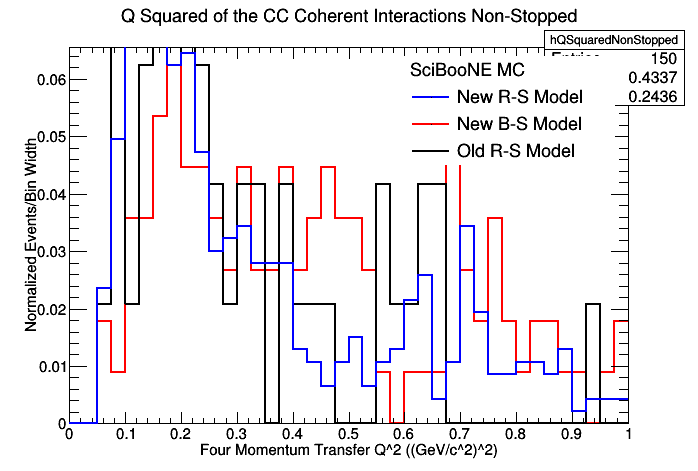
\includegraphics[width=0.6\textwidth]{NMFourSquaredPlottingImages/1-NMFourSquaredPlotting.png}
\caption{}
\end{figure}

\begin{figure}[H]
\centering
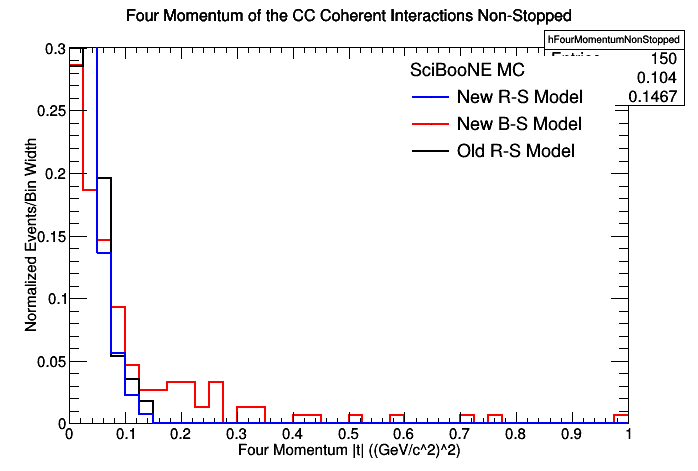
\includegraphics[width=0.6\textwidth]{NMFourSquaredPlottingImages/2-NMFourSquaredPlotting.png}
\caption{}
\end{figure}

\begin{figure}[H]
\centering
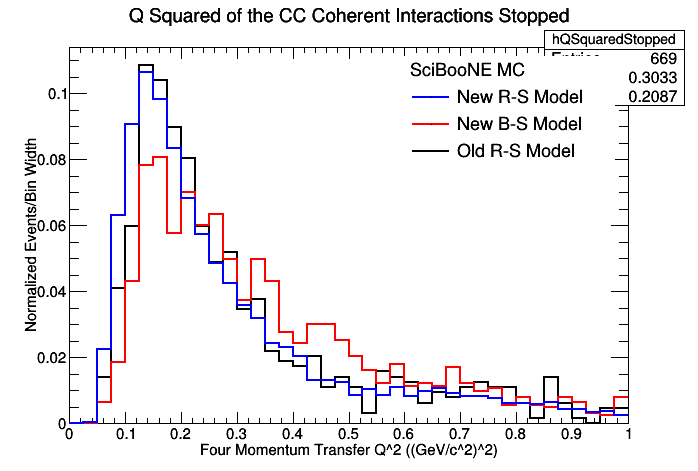
\includegraphics[width=0.6\textwidth]{NMFourSquaredPlottingImages/3-NMFourSquaredPlotting.png}
\caption{}
\end{figure}

\begin{figure}[H]
\centering
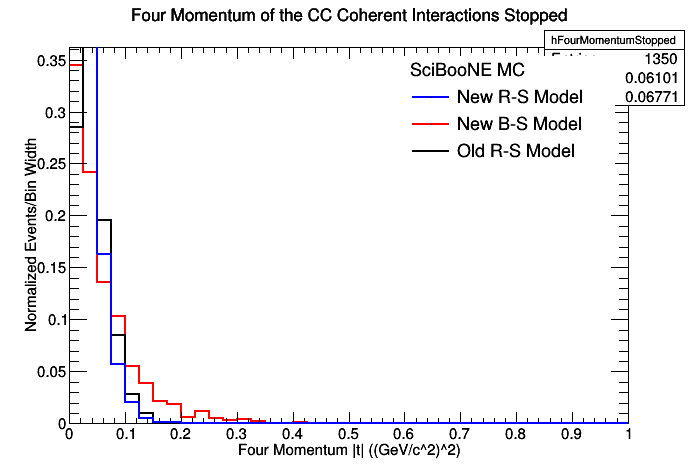
\includegraphics[width=0.6\textwidth]{NMFourSquaredPlottingImages/4-NMFourSquaredPlotting.png}
\caption{}
\end{figure}

\begin{figure}[H]
\centering
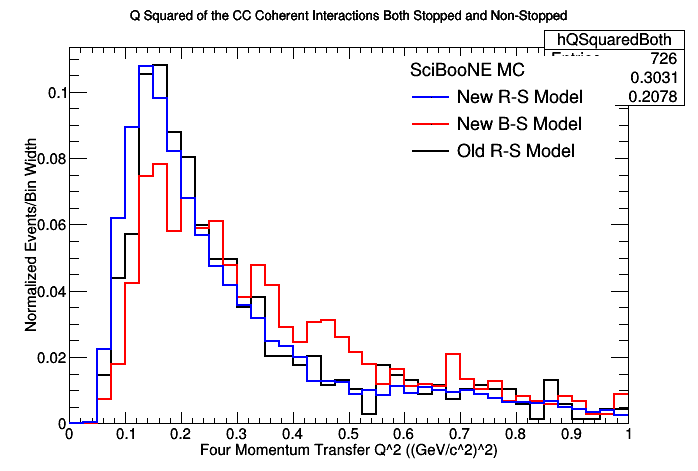
\includegraphics[width=0.6\textwidth]{NMFourSquaredPlottingImages/5-NMFourSquaredPlotting.png}
\caption{}
\end{figure}

\begin{figure}[H]
\centering
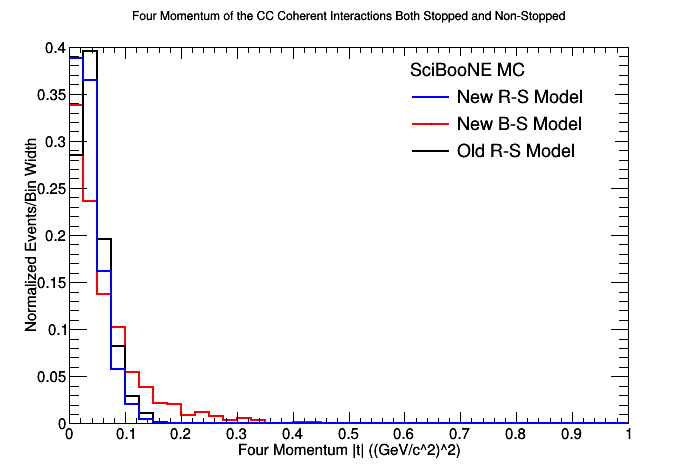
\includegraphics[width=0.6\textwidth]{NMFourSquaredPlottingImages/6-NMFourSquaredPlotting.png}
\caption{}
\end{figure}

$\bar{\nu}$-Mode $|t|$ and $Q^2$ plots are below:
\begin{figure}[H]
\centering
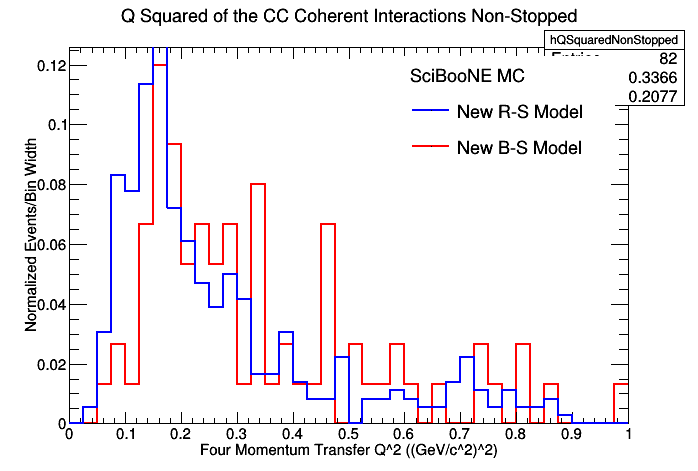
\includegraphics[width=0.6\textwidth]{ANMFourSquaredPlottingImages/1-ANMFourSquaredPlotting.png}
\caption{}
\end{figure}

\begin{figure}[H]
\centering
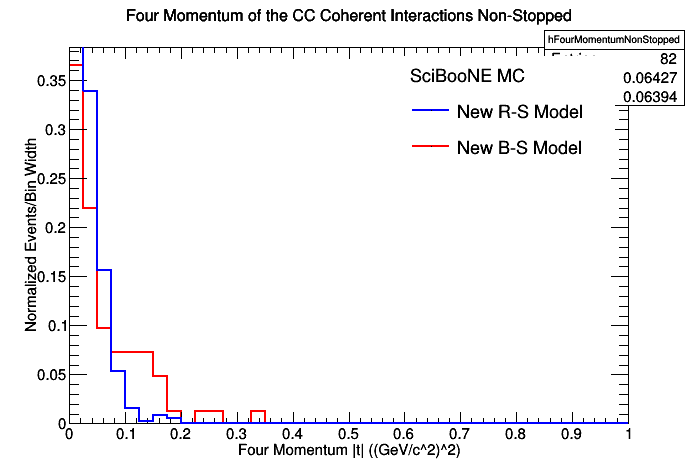
\includegraphics[width=0.6\textwidth]{ANMFourSquaredPlottingImages/2-ANMFourSquaredPlotting.png}
\caption{}
\end{figure}

\begin{figure}[H]
\centering
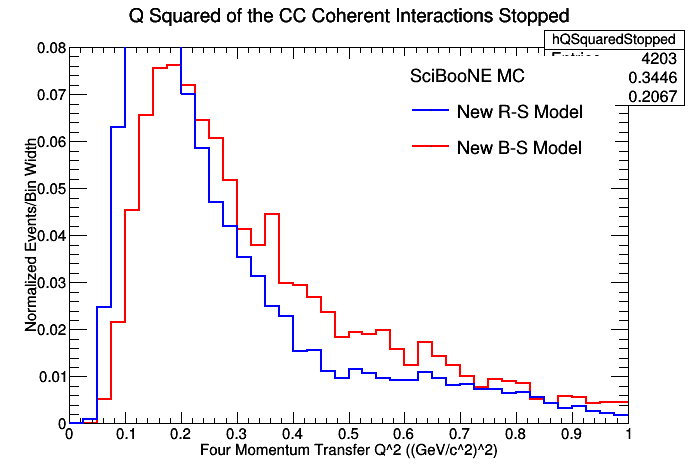
\includegraphics[width=0.6\textwidth]{ANMFourSquaredPlottingImages/3-ANMFourSquaredPlotting.png}
\caption{}
\end{figure}

\begin{figure}[H]
\centering
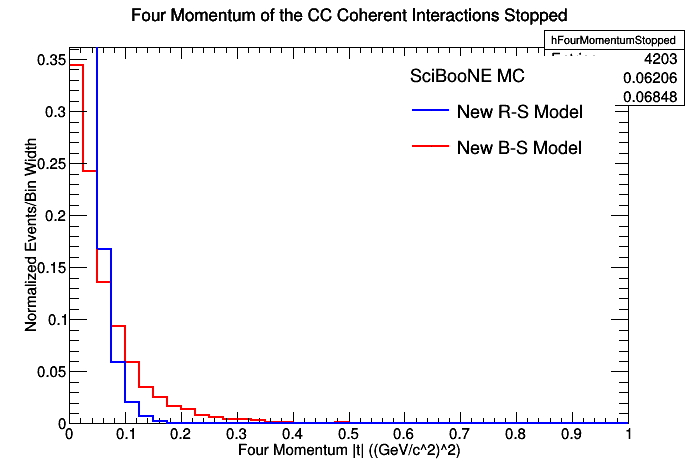
\includegraphics[width=0.6\textwidth]{ANMFourSquaredPlottingImages/4-ANMFourSquaredPlotting.png}
\caption{}
\end{figure}

\begin{figure}[H]
\centering
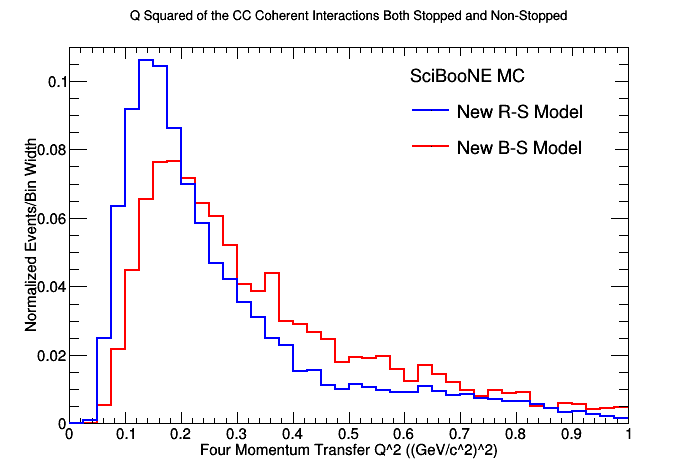
\includegraphics[width=0.6\textwidth]{ANMFourSquaredPlottingImages/5-ANMFourSquaredPlotting.png}
\caption{}
\end{figure}

\begin{figure}[H]
\centering
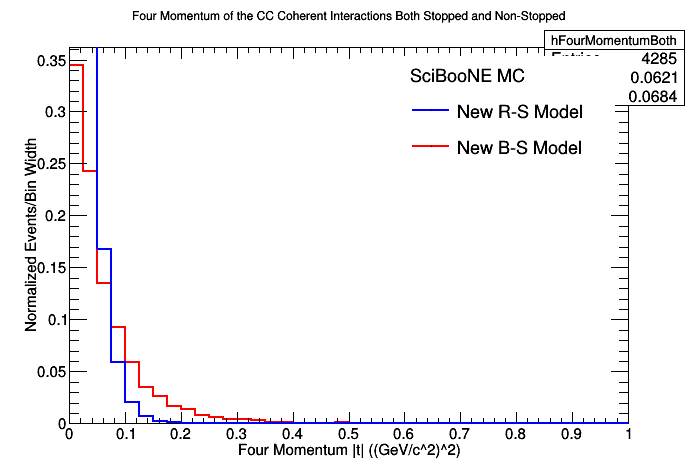
\includegraphics[width=0.6\textwidth]{ANMFourSquaredPlottingImages/6-ANMFourSquaredPlotting.png}
\caption{}
\end{figure}
% This is where the t and q2 plots end


%=========================================================================
%=========================================================================
%
%=========================================================================
%=========================================================================
\newpage

\appendix


%=========================================================================
\section{Appendix: Sample Details}\label{sec:SampleAppendix}
%=========================================================================

Appendix on samples

%-----------------------------------------------------------------------------------------------------------------|
\subsection{$\nu$-Mode Rein-Sehgal NEUTv5.3.6}
A sample of 1,000,000 $\nu$ interactions were simulated using the NEUT generator (v5.3.6) and the Rein-Sehgal model for coherent pion production. This sample correspond to the file labeled 
\begin{verbatim}
SciBooNE_numu_coh_RooTrack.root
\end{verbatim}
found at the following link (put link to sample here).

%-----------------------------------------------------------------------------------------------------------------|
\subsection{$\nu$-Mode Berger-Sehgal NEUTv5.3.6}
A sample of 1,000,000 $\nu$ interactions were simulated using the NEUT generator (v5.3.6) and the Berger-Sehgal model for coherent pion production. This sample correspond to the file labeled
\begin{verbatim}
SciBooNE_numu_coh_RooTrack_NEW.root
\end{verbatim}
found at the following link (put link to sample here).



%-----------------------------------------------------------------------------------------------------------------|
\subsection{$\nu$-Mode Rein-Sehgal NEUTvx.x.x}
A sample of 100,000 $\nu$ interactions were simulated using the NEUT generator (vx.x.x, believed to be the version used by the SciBooNE collaboration in the original publication) and the corresponding older Rein-Sehgal model for coherent pion production. This sample correspond to the file labeled
\begin{verbatim}
SciBooNE_numu_coh_OLDNEUT_RooTrack.root
\end{verbatim}
found at the following link (put link to sample here).


%-----------------------------------------------------------------------------------------------------------------|
\subsection{$bar{\nu}$-Mode Rein-Sehgal NEUTv5.3.6}
A sample of 1,000,000 $\bar{\nu}$ interactions were simulated using the NEUT generator (v5.3.6) and the Rein-Sehgal model for coherent pion production. This sample correspond to the file labeled
\begin{verbatim}
SciBooNE_numubar_coh_RooTrack.root
\end{verbatim}
found at the following link (put link to sample here).

%-----------------------------------------------------------------------------------------------------------------|
\subsection{$\bar{\nu}$-Mode Berger-Sehgal NEUTv5.3.6}
A sample of 1,000,000 $\bar{\nu}$ interactions were simulated using the NEUT generator (v5.3.6) and the Berger-Sehgal model for coherent pion production. This sample correspond to the file labeled
\begin{verbatim}
SciBooNE_numubar_coh_RooTrack_NEW.root
\end{verbatim}
found at the following link (put link to sample here).




%-----------------------------------------------------------------------------------------------------------------|
\subsection{Vertex Distributions}
The events were all given a random initial point that was generated with the goal that the vertex distributions of this simulation would closely match the vertex distributions that Hiraide (need to put a reference) showed in his thesis. This was done by... etc.

\begin{lstlisting}[language=C]
Put in the code for how we made the vertex distributions of the interactions.
\end{lstlisting}

\begin{figure}[H]
\centering
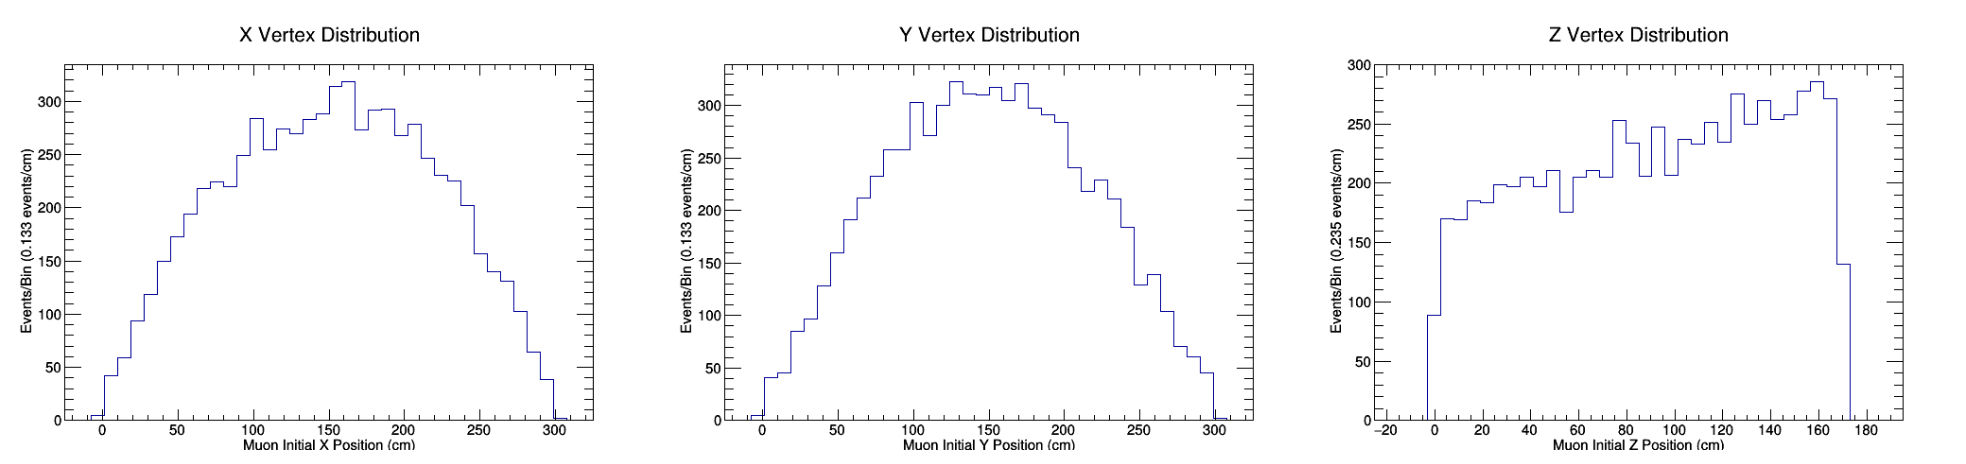
\includegraphics[width=1.0\textwidth]{EventClassifications/VertexDistributions.png}
\caption{Vertex distributions of the events in the new Rein-Sehgal sample.}
\end{figure}






%-----------------------------------------------------------------------------------------------------------------|
\subsection{NewNMReinSehgal.C}
This file is the macro that corresponds to the "NewNMReinSehgal.h" file, which connects with this file: "SciBooNE\textunderscore numu\textunderscore coh\textunderscore RooTrack.root". This file performs the main analysis for this generated sample, and then organizes the information into many different histograms. The histograms are then written to a file titled "totalmuoninfoRS.root" inside the "ROOTFILES" directory. The "ROOTFILES" directory is included in the SciBooNE-MC repository (it is absolutely pertinent that this directory be located where the macro files are located due to how the calls of the combined data macros reference the now saved histograms). When this macro is run (which can take a while), it also plots a few different histograms. The histograms that are plotted are the ones shown in the figures below with descriptions included with the corresponding figures. The order that the histograms appear in this paper is the same order they will be shown when this macro is run in root.

\begin{figure}[H]
\centering
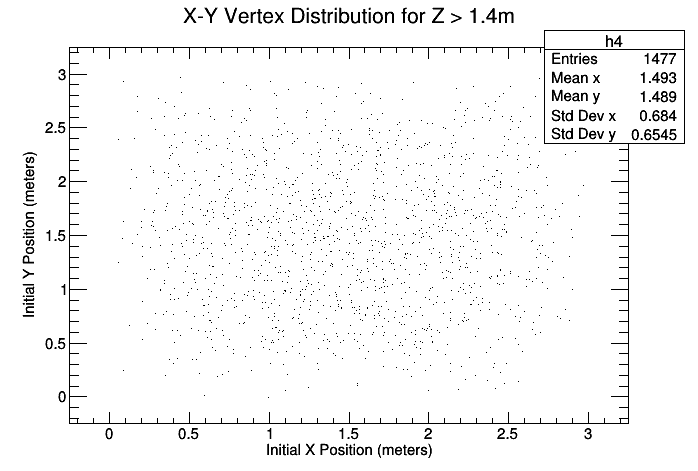
\includegraphics[width=0.6\textwidth]{NewNMReinSehgalImages/1-X-YVertexDistributionNMRS.png}
\caption{New $\nu$-Mode Rein-Sehgal X-Y vertex distributions for muons that made it to the MRD and penetrated at least to the third layer of steel.}
\end{figure}

\begin{figure}[H]
\centering
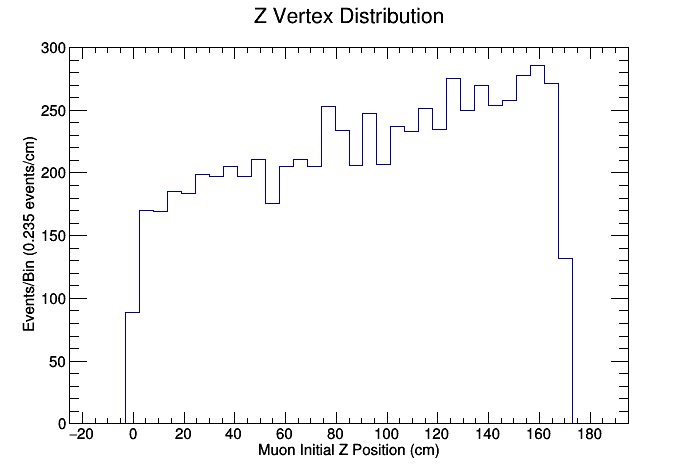
\includegraphics[width=0.6\textwidth]{NewNMReinSehgalImages/2-ZVertexDistributionNMRS.png}
\caption{New $\nu$-Mode Rein-Sehgal Z vertex distributions for the interactions.}
\end{figure}

\begin{figure}[H]
\centering
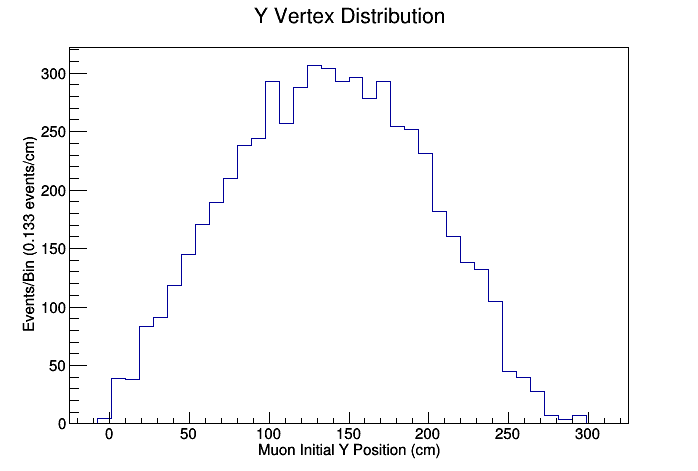
\includegraphics[width=0.6\textwidth]{NewNMReinSehgalImages/3-YVertexDistributionNMRS.png}
\caption{New $\nu$-Mode Rein-Sehgal Y vertex distributions for the interactions.}
\end{figure}

\begin{figure}[H]
\centering
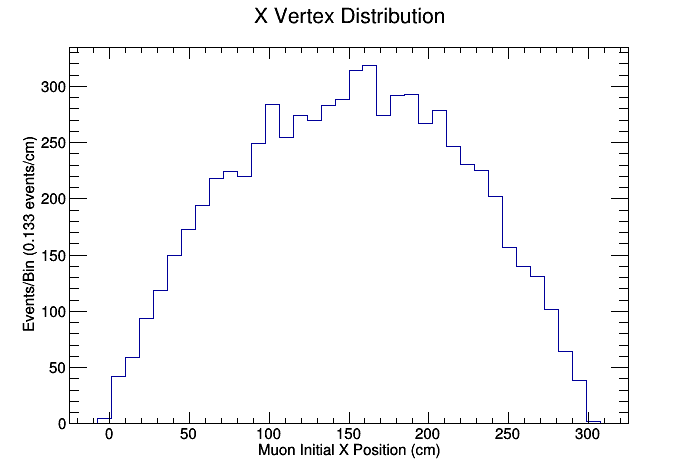
\includegraphics[width=0.6\textwidth]{NewNMReinSehgalImages/4-XVertexDistributionNMRS.png}
\caption{New $\nu$-Mode Rein-Sehgal X vertex distributions for the interactions.}
\end{figure}

\begin{figure}[H]
\centering
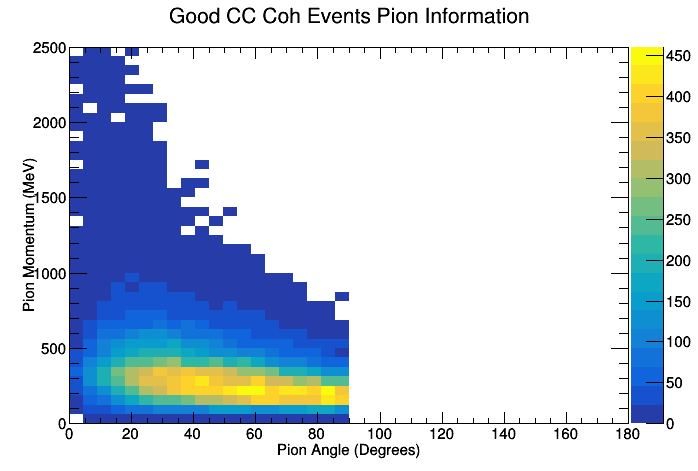
\includegraphics[width=0.6\textwidth]{NewNMReinSehgalImages/5-GoodCCCohPionInfoNMRS.png}
\caption{This is a 2D histogram for the momentum and angle of the pion in the CC Coh Pion events that met the qualification of being "good".}
\end{figure}

\begin{figure}[H]
\centering
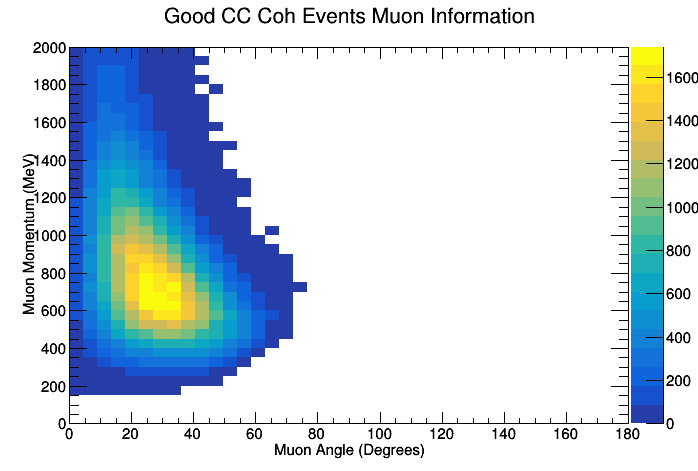
\includegraphics[width=0.6\textwidth]{NewNMReinSehgalImages/6-GoodCCCohMuonInfoNMRS.png}
\caption{This is a 2D histogram for the momentum and angle of the muon in the CC Coh Pion events that met the qualification of being "good".}
\end{figure}

\begin{figure}[H]
\centering
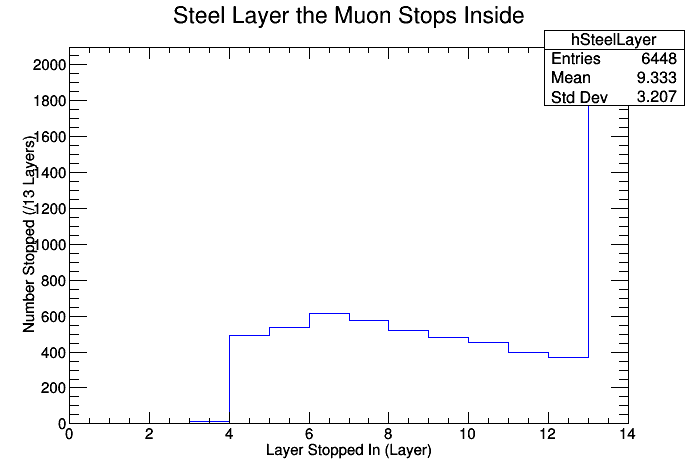
\includegraphics[width=0.6\textwidth]{NewNMReinSehgalImages/7-LayerPenetrationNMRS.png}
\caption{This histogram shows the amount of muons that embedded (or "Stopped") in a corresponding layer of steel in our simulation.}
\end{figure}

\begin{figure}[H]
\centering
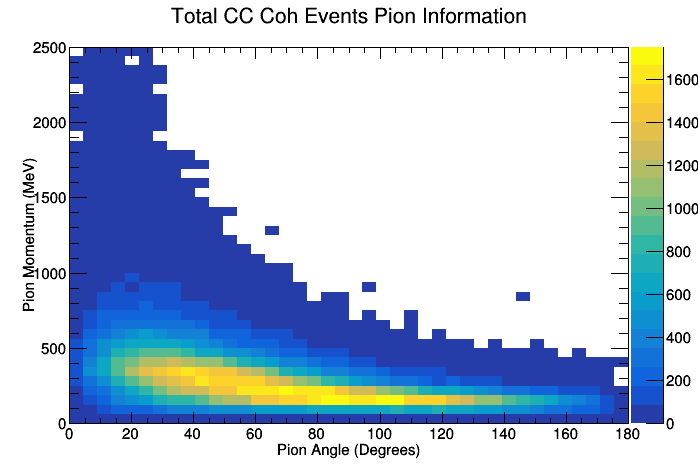
\includegraphics[width=0.6\textwidth]{NewNMReinSehgalImages/8-TotalCCCohPionInfoNMRS.png}
\caption{This is a 2D histogram for the momentum and angle of the pion in the total CC Coh Pion events.}
\end{figure}

\begin{figure}[H]
\centering
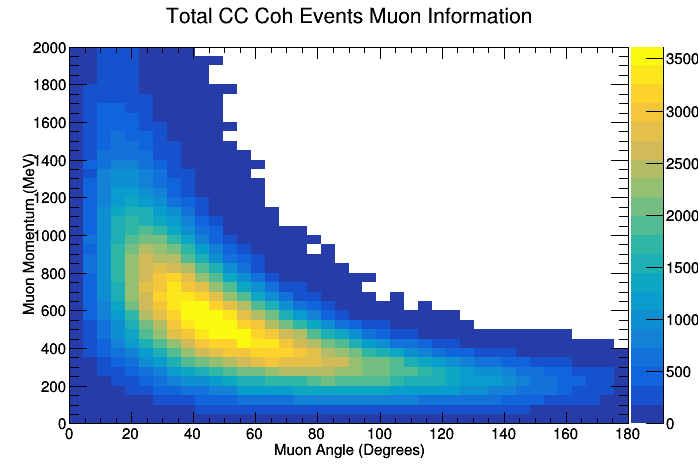
\includegraphics[width=0.6\textwidth]{NewNMReinSehgalImages/9-TotalCCCohMuonInfoNMRS.png}
\caption{This is a 2D histogram for the momentum and angle of the muon in the total CC Coh Pion events.}
\end{figure}

The NewNMReinSehgal.C macro also calculates many different quantities for the generated simulation of the events and saves the information in histograms that are later called upon through the plotting macros (which are after all of the analysis macros). The first quantity that is calculated for the different vertexes is the momentum of both the muon and the pion, which are both calculated using the equations:

\begin{equation}
|\vec{p}_\mu| = \sqrt{P_{\mu_x}^2 + P_{\mu_y}^2 + P_{\mu_z}^2}
\end{equation}

\begin{equation}
|\vec{p}_\pi| = \sqrt{P_{\pi_x}^2 + P_{\pi_y}^2 + P_{\pi_z}^2}
\end{equation}

\noindent
The momentum is reported in units of $MeV/c$.

The next quantity that is calculated in the macro is the angle from the beam-direction for both the muon and the pion, which are labeled as either $\theta_\mu$, or $\theta_\pi$, respectively. The angle from the beam-direction is the same as the angle from the z-direction, and this angle is known as the azimuthal angle. The calculation of the azimuthal angle is slightly more involved than the simple calculation used for finding the magnitude of the momentum of the two particles, and is calculated using the equations:

\begin{equation}
\theta_\mu = tan^{-1}(\sqrt{P_{\mu_x}^2 + P_{\mu_y}^2}/{P_{\mu_z}})
\end{equation}

\begin{equation}
\theta_\pi = tan^{-1}(\sqrt{P_{\pi_x}^2 + P_{\pi_y}^2}/{P_{\pi_z}})
\end{equation}

\noindent
The angles are reported in units of $\degree$, and should run from $0\degree$ to $180\degree$. In the case of Charged-Current Coherent Pion Production, the angle should never be larger than $90\degree$.

The last two quantities that this analysis macro calculates are the two different types of four-momentum transfers specific to this interaction, which are $Q^2$ and $|t|$. The $Q^2$ corresponds to the four-momentum transfer from the neutrino and muon to the nucleus and pion, and is calculated using the equation:

\begin{equation}
Q^2 = |(P_{\nu_\mu} - P_\mu)^2|
\end{equation}

\noindent
This equation is the four-momentum notational form. The code follows the equation below in order to compute $Q^2$:

\begin{equation}
Q^2 = |(P_{\nu_{\mu,x}} - P_{\mu_x})^2 + (P_{\nu_{\mu,y}} - P_{\mu_y})^2 + (P_{\nu_{\mu,z}} - P_{\mu_z})^2 + (P_{\nu_{\mu,E}} - P_{\mu_E})^2|
\end{equation}

\noindent
$Q^2$ is reported in units of $(MeV/c)^2$.

The $|t|$ corresponds to the four-momentum transfer from the neutrino, muon, and pion to the nucleus, and is calculated using the equation:

\begin{equation}
|t| = |(Q - P_\pi)^2| = |(P_{\nu_\mu} - P_\mu - P_\pi)^2|
\end{equation}

\noindent
This equation is the four-momentum notational form. The code follows the equation below in order to compute $|t|$:

\begin{equation}
|t| = |(P_{\nu_{\mu,x}} - P_{\mu_x} - P_{\pi_x})^2 + (P_{\nu_{\mu,y}} - P_{\mu_y} - P_{\pi_y})^2 + (P_{\nu_{\mu,z}} - P_{\mu_z} - P_{\pi_z})^2 + (P_{\nu_{\mu,E}} - P_{\mu_E} - P_{\pi_E})^2|
\end{equation}

\noindent
$|t|$ is reported in units of $(MeV/c)^2$.

%-----------------------------------------------------------------------------------------------------------------|
\subsection{NewNMBergerSehgal.C}
This file is the macro that corresponds to the "NewNMBergerSehgal.h" file, which connects with this file: "SciBooNE\textunderscore numu\textunderscore coh\textunderscore RooTrack\textunderscore NEW.root". This file performs the main analysis for this generated sample, and then organizes the information into many different histograms. The histograms are then written to a file titled "totalmuoninfoBS.root" inside the "ROOTFILES" directory. The "ROOTFILES" directory is included in the SciBooNE-MC repository (it is absolutely pertinent that this directory be located where the macro files are located due to how the calls of the combined data macros reference the now saved histograms).

\begin{figure}[H]
\centering
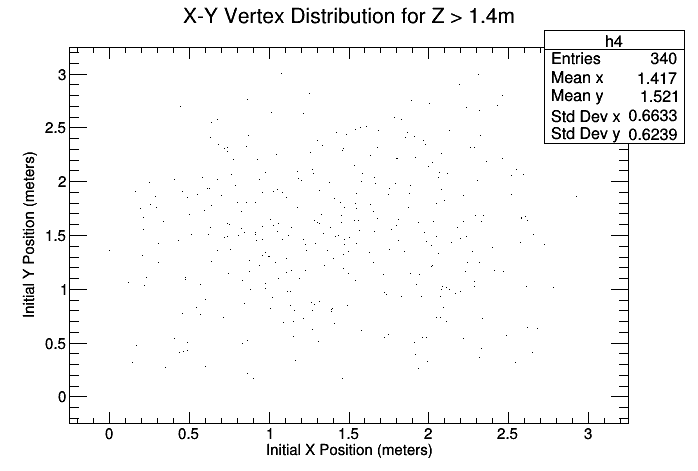
\includegraphics[width=0.6\textwidth]{NewNMBergerSehgalImages/1-X-YVertexDistributionNMBS.png}
\caption{New $\nu$-Mode Berger-Sehgal X-Y vertex distributions for muons that made it to the MRD and penetrated at least to the third layer of steel.}
\end{figure}

\begin{figure}[H]
\centering
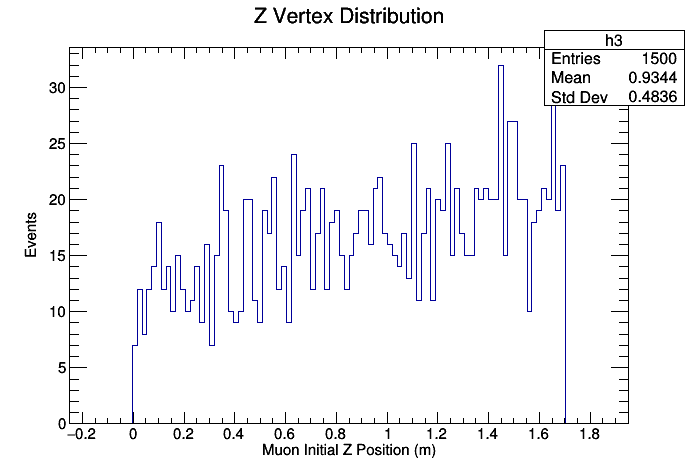
\includegraphics[width=0.6\textwidth]{NewNMBergerSehgalImages/2-ZVertexDistributionNMBS.png}
\caption{New $\nu$-Mode Berger-Sehgal Z vertex distributions for the interactions.}
\end{figure}

\begin{figure}[H]
\centering
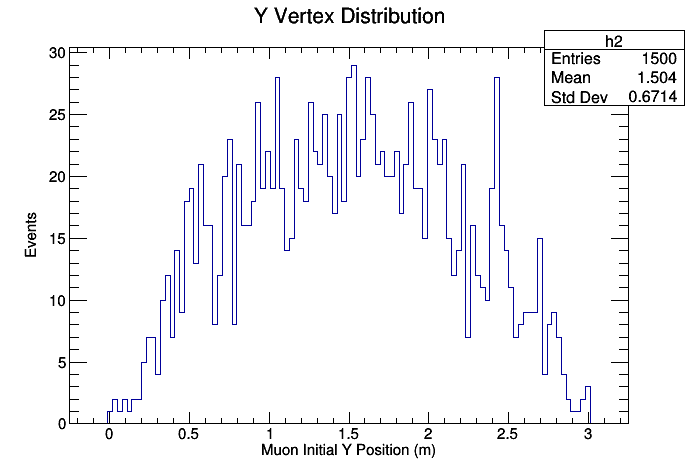
\includegraphics[width=0.6\textwidth]{NewNMBergerSehgalImages/3-YVertexDistributionNMBS.png}
\caption{New $\nu$-Mode Berger-Sehgal Y vertex distributions for the interactions.}
\end{figure}

\begin{figure}[H]
\centering
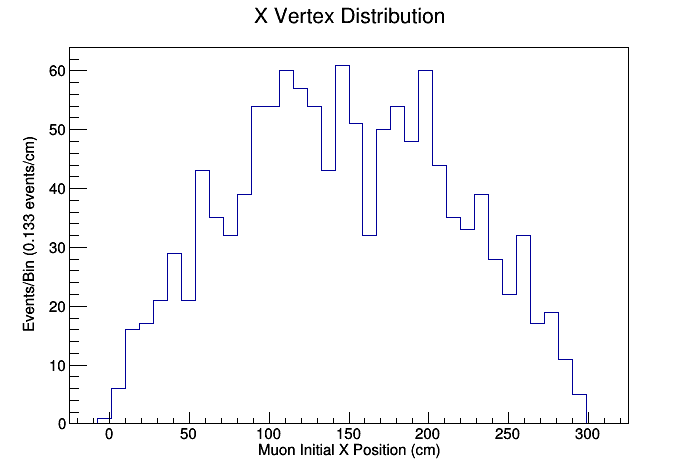
\includegraphics[width=0.6\textwidth]{NewNMBergerSehgalImages/4-XVertexDistributionNMBS.png}
\caption{New $\nu$-Mode Berger-Sehgal X vertex distributions for the interactions.}
\end{figure}

\begin{figure}[H]
\centering
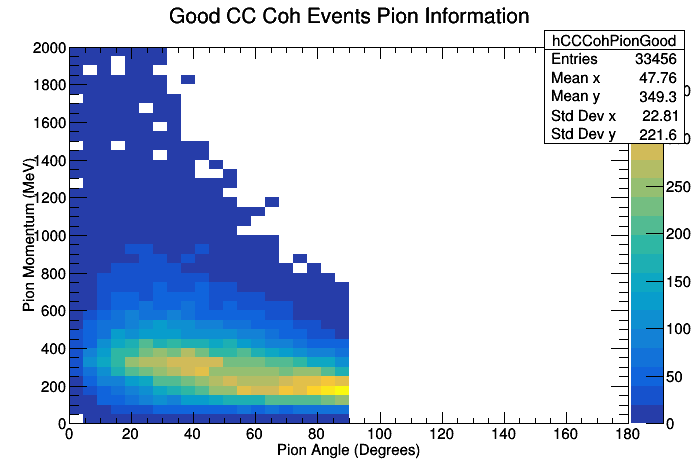
\includegraphics[width=0.6\textwidth]{NewNMBergerSehgalImages/5-GoodCCCohPionInfoNMBS.png}
\caption{This is a 2D histogram for the momentum and angle of the pion in the CC Coh Pion events that met the qualification of being "good".}
\end{figure}

\begin{figure}[H]
\centering
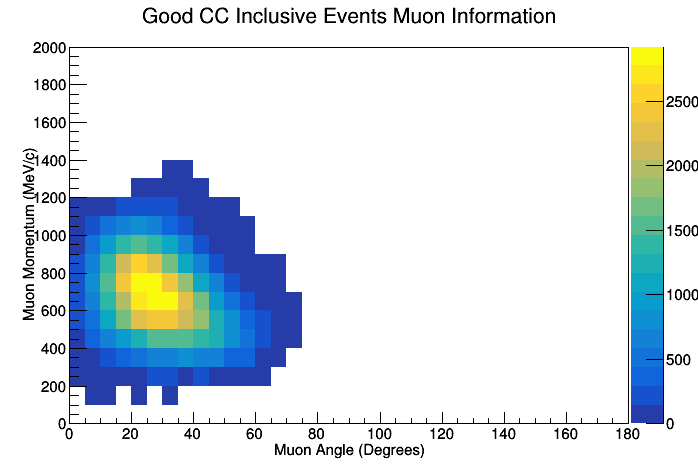
\includegraphics[width=0.6\textwidth]{NewNMBergerSehgalImages/6-GoodCCCohMuonInfoNMBS.png}
\caption{This is a 2D histogram for the momentum and angle of the muon in the CC Coh Pion events that met the qualification of being "good".!}
\end{figure}

\begin{figure}[H]
\centering
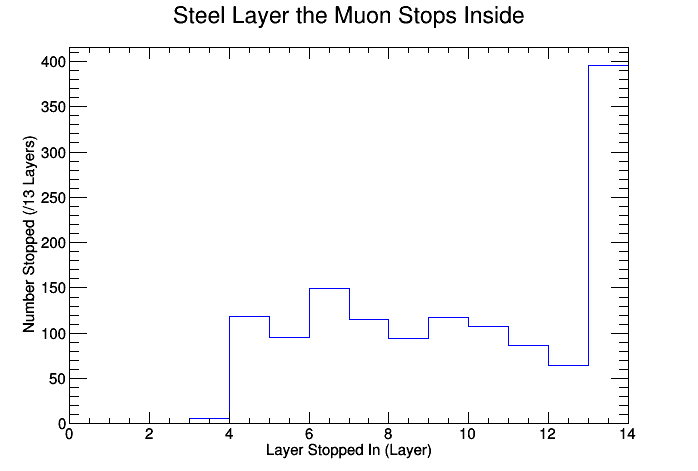
\includegraphics[width=0.6\textwidth]{NewNMBergerSehgalImages/7-LayerPenetrationNMBS.png}
\caption{This histogram shows the amount of muons that embedded (or "Stopped") in a corresponding layer of steel in our simulation.}
\end{figure}

\begin{figure}[H]
\centering
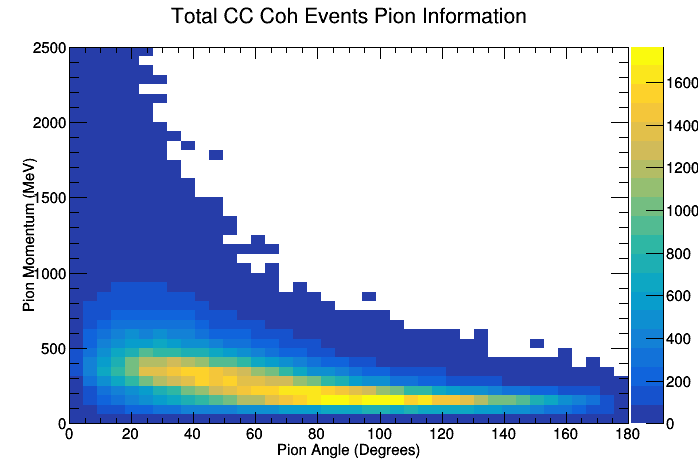
\includegraphics[width=0.6\textwidth]{NewNMBergerSehgalImages/8-TotalCCCohPionInfoNMBS.png}
\caption{This is a 2D histogram for the momentum and angle of the pion in the total CC Coh Pion events.}
\end{figure}

\begin{figure}[H]
\centering
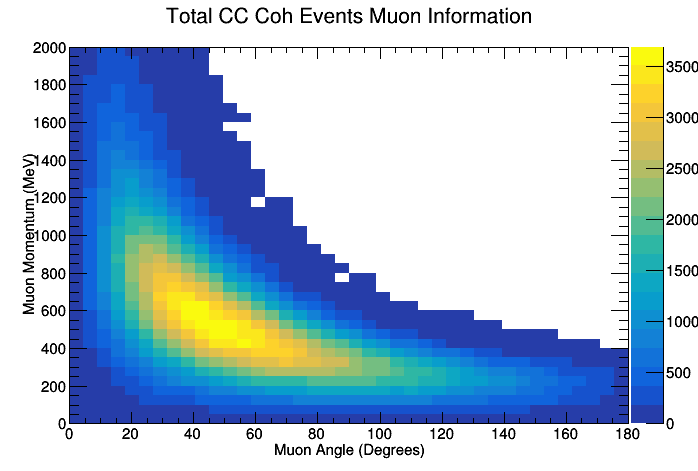
\includegraphics[width=0.6\textwidth]{NewNMBergerSehgalImages/9-TotalCCCohMuonInfoNMBS.png}
\caption{This is a 2D histogram for the momentum and angle of the muon in the total CC Coh Pion events.}
\end{figure}

The NewNMBergerSehgal.C macro also calculates many different quantities for the generated simulation of the events and saves the information in histograms that are later called upon through the plotting macros (which are after all of the analysis macros). The first quantity that is calculated for the different vertexes is the momentum of both the muon and the pion, which are both calculated using the equations:

\begin{equation}
|\vec{p}_\mu| = \sqrt{P_{\mu_x}^2 + P_{\mu_y}^2 + P_{\mu_z}^2}
\end{equation}

\begin{equation}
|\vec{p}_\pi| = \sqrt{P_{\pi_x}^2 + P_{\pi_y}^2 + P_{\pi_z}^2}
\end{equation}

\noindent
The momentum is reported in units of $MeV/c$.

The next quantity that is calculated in the macro is the angle from the beam-direction for both the muon and the pion, which are labeled as either $\theta_\mu$, or $\theta_\pi$, respectively. The angle from the beam-direction is the same as the angle from the z-direction, and this angle is known as the azimuthal angle. The calculation of the azimuthal angle is slightly more involved than the simple calculation used for finding the magnitude of the momentum of the two particles, and is calculated using the equations:

\begin{equation}
\theta_\mu = tan^{-1}(\sqrt{P_{\mu_x}^2 + P_{\mu_y}^2}/{P_{\mu_z}})
\end{equation}

\begin{equation}
\theta_\pi = tan^{-1}(\sqrt{P_{\pi_x}^2 + P_{\pi_y}^2}/{P_{\pi_z}})
\end{equation}

\noindent
The angles are reported in units of $\degree$, and should run from $0\degree$ to $180\degree$. In the case of Charged-Current Coherent Pion Production, the angle should never be larger than $90\degree$.

The last two quantities that this analysis macro calculates are the two different types of four-momentum transfers specific to this interaction, which are $Q^2$ and $|t|$. The $Q^2$ corresponds to the four-momentum transfer from the neutrino and muon to the nucleus and pion, and is calculated using the equation:

\begin{equation}
Q^2 = |(P_{\nu_\mu} - P_\mu)^2|
\end{equation}

\noindent
This equation is the four-momentum notational form. The code follows the equation below in order to compute $Q^2$:

\begin{equation}
Q^2 = |(P_{\nu_{\mu,x}} - P_{\mu_x})^2 + (P_{\nu_{\mu,y}} - P_{\mu_y})^2 + (P_{\nu_{\mu,z}} - P_{\mu_z})^2 + (P_{\nu_{\mu,E}} - P_{\mu_E})^2|
\end{equation}

\noindent
$Q^2$ is reported in units of $(MeV/c)^2$.

The $|t|$ corresponds to the four-momentum transfer from the neutrino, muon, and pion to the nucleus, and is calculated using the equation:

\begin{equation}
|t| = |(Q - P_\pi)^2| = |(P_{\nu_\mu} - P_\mu - P_\pi)^2|
\end{equation}

\noindent
This equation is the four-momentum notational form. The code follows the equation below in order to compute $|t|$:

\begin{equation}
|t| = |(P_{\nu_{\mu,x}} - P_{\mu_x} - P_{\pi_x})^2 + (P_{\nu_{\mu,y}} - P_{\mu_y} - P_{\pi_y})^2 + (P_{\nu_{\mu,z}} - P_{\mu_z} - P_{\pi_z})^2 + (P_{\nu_{\mu,E}} - P_{\mu_E} - P_{\pi_E})^2|
\end{equation}

\noindent
$|t|$ is reported in units of $(MeV/c)^2$.

%-----------------------------------------------------------------------------------------------------------------|
\subsection{OldNMReinSehgal.C}
This file is the macro that corresponds to the "OldNMReinSehgal.h" file, which connects with this file: "SciBooNE\textunderscore numu\textunderscore coh\textunderscore OLDNEUT\textunderscore RooTrack.root". This file performs the main analysis for this generated sample, and then organizes the information into many different histograms. The histograms are then written to a file titled "totalmuoninfoOBS.root" inside the "ROOTFILES" directory. The "ROOTFILES" directory is included in the SciBooNE-MC repository (it is absolutely pertinent that this directory be located where the macro files are located due to how the calls of the combined data macros reference the now saved histograms).

\begin{figure}[H]
\centering
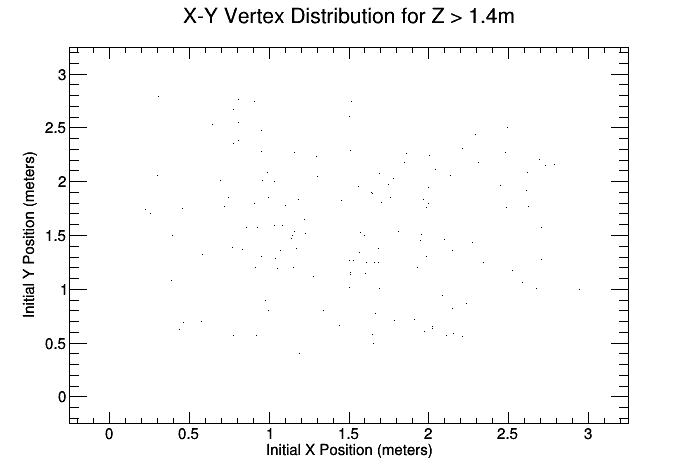
\includegraphics[width=0.6\textwidth]{OldNMReinSehgalImages/1-X-YVertexDistributionNMORS.png}
\caption{Old $\nu$-Mode Rein-Sehgal X-Y vertex distributions for muons that made it to the MRD and penetrated at least to the third layer of steel.}
\end{figure}

\begin{figure}[H]
\centering
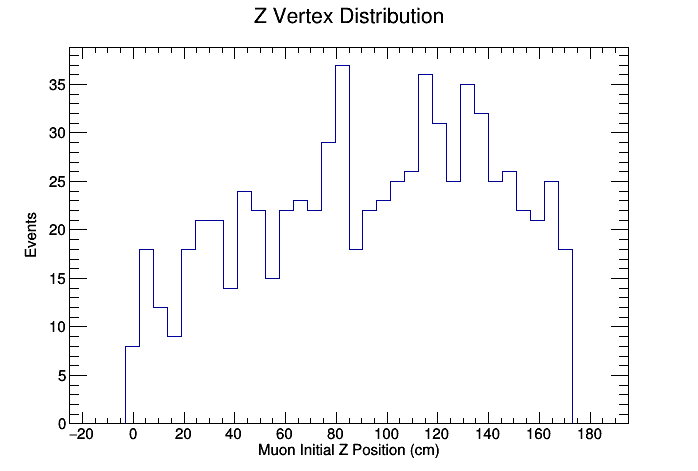
\includegraphics[width=0.6\textwidth]{OldNMReinSehgalImages/2-ZVertexDistributionNMORS.png}
\caption{Old $\nu$-Mode Rein-Sehgal Z vertex distributions for the interactions.}
\end{figure}

\begin{figure}[H]
\centering
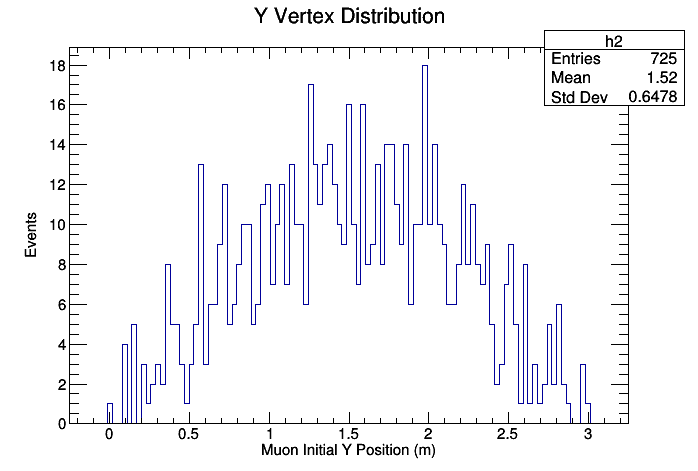
\includegraphics[width=0.6\textwidth]{OldNMReinSehgalImages/3-YVertexDistributionNMORS.png}
\caption{Old $\nu$-Mode Rein-Sehgal Y vertex distributions for the interactions.}
\end{figure}

\begin{figure}[H]
\centering
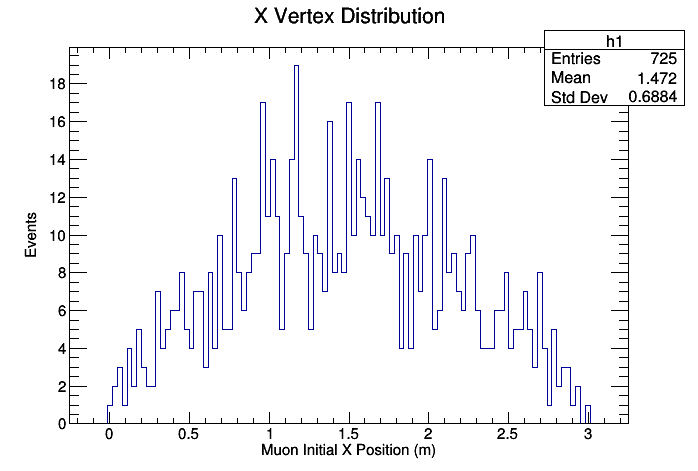
\includegraphics[width=0.6\textwidth]{OldNMReinSehgalImages/4-XVertexDistributionNMORS.png}
\caption{Old $\nu$-Mode Rein-Sehgal X vertex distributions for the interactions.}
\end{figure}

\begin{figure}[H]
\centering
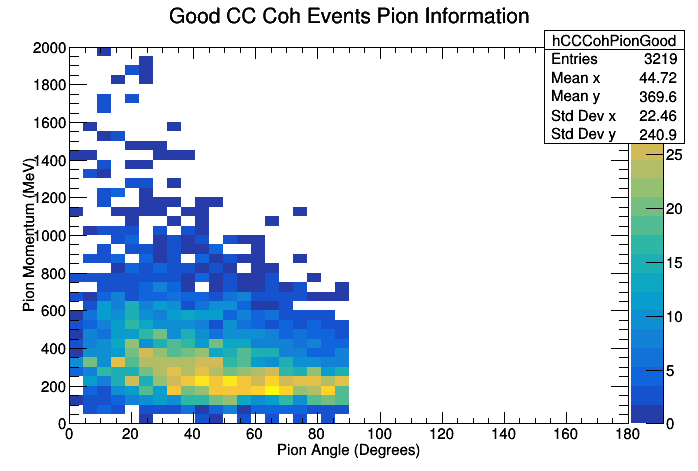
\includegraphics[width=0.6\textwidth]{OldNMReinSehgalImages/5-GoodCCCohPionInfoNMORS.png}
\caption{This is a 2D histogram for the momentum and angle of the pion in the CC Coh Pion events that met the qualification of being "good".}
\end{figure}

\begin{figure}[H]
\centering
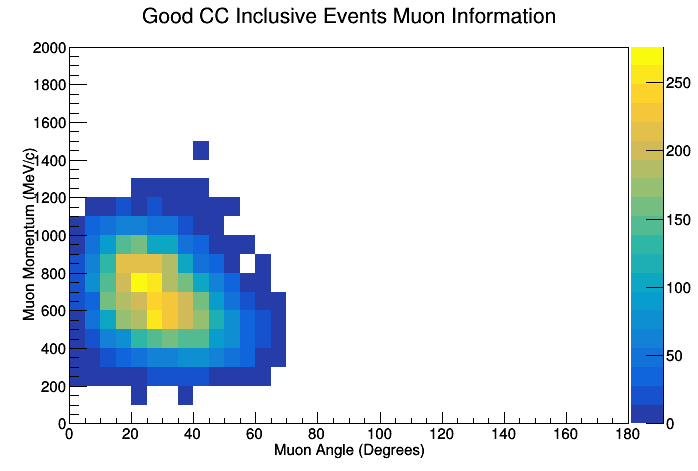
\includegraphics[width=0.6\textwidth]{OldNMReinSehgalImages/6-GoodCCCohMuonInfoNMORS.png}
\caption{This is a 2D histogram for the momentum and angle of the muon in the CC Coh Pion events that met the qualification of being "good".}
\end{figure}

\begin{figure}[H]
\centering
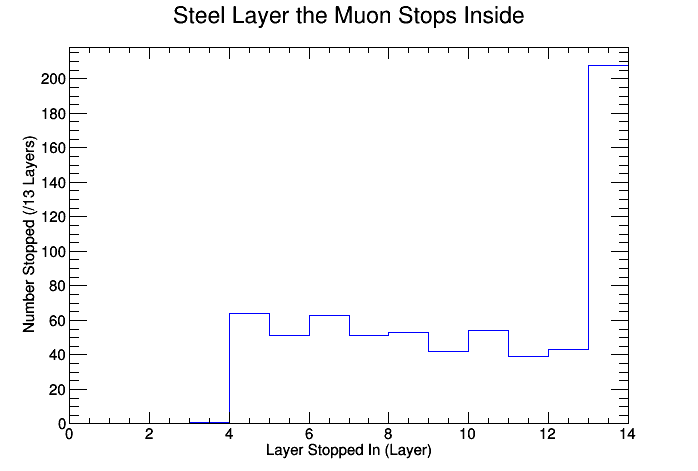
\includegraphics[width=0.6\textwidth]{OldNMReinSehgalImages/7-LayerPenetrationNMORS.png}
\caption{This histogram shows the amount of muons that embedded (or "Stopped") in a corresponding layer of steel in our simulation.}
\end{figure}

\begin{figure}[H]
\centering
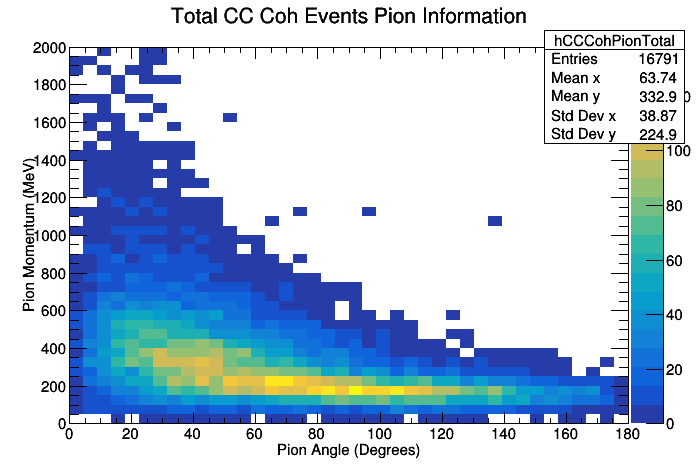
\includegraphics[width=0.6\textwidth]{OldNMReinSehgalImages/8-TotalCCCohPionInfoNMORS.png}
\caption{This is a 2D histogram for the momentum and angle of the pion in the total CC Coh Pion events.}
\end{figure}

\begin{figure}[H]
\centering
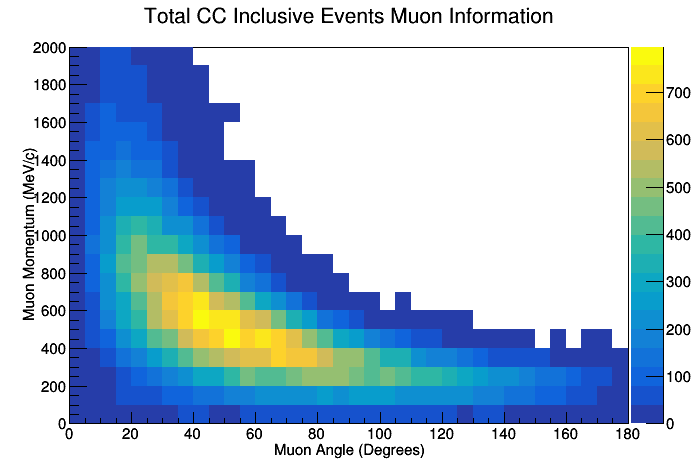
\includegraphics[width=0.6\textwidth]{OldNMReinSehgalImages/9-TotalCCCohMuonInfoNMORS.png}
\caption{This is a 2D histogram for the momentum and angle of the muon in the total CC Coh Pion events.}
\end{figure}

The OldNMReinSehgal.C macro also calculates many different quantities for the generated simulation of the events and saves the information in histograms that are later called upon through the plotting macros (which are after all of the analysis macros). The first quantity that is calculated for the different vertexes is the momentum of both the muon and the pion, which are both calculated using the equations:

\begin{equation}
|\vec{p}_\mu| = \sqrt{P_{\mu_x}^2 + P_{\mu_y}^2 + P_{\mu_z}^2}
\end{equation}

\begin{equation}
|\vec{p}_\pi| = \sqrt{P_{\pi_x}^2 + P_{\pi_y}^2 + P_{\pi_z}^2}
\end{equation}

\noindent
The momentum is reported in units of $MeV/c$.

The next quantity that is calculated in the macro is the angle from the beam-direction for both the muon and the pion, which are labeled as either $\theta_\mu$, or $\theta_\pi$, respectively. The angle from the beam-direction is the same as the angle from the z-direction, and this angle is known as the azimuthal angle. The calculation of the azimuthal angle is slightly more involved than the simple calculation used for finding the magnitude of the momentum of the two particles, and is calculated using the equations:

\begin{equation}
\theta_\mu = tan^{-1}(\sqrt{P_{\mu_x}^2 + P_{\mu_y}^2}/{P_{\mu_z}})
\end{equation}

\begin{equation}
\theta_\pi = tan^{-1}(\sqrt{P_{\pi_x}^2 + P_{\pi_y}^2}/{P_{\pi_z}})
\end{equation}

\noindent
The angles are reported in units of $\degree$, and should run from $0\degree$ to $180\degree$. In the case of Charged-Current Coherent Pion Production, the angle should never be larger than $90\degree$.

The last two quantities that this analysis macro calculates are the two different types of four-momentum transfers specific to this interaction, which are $Q^2$ and $|t|$. The $Q^2$ corresponds to the four-momentum transfer from the neutrino and muon to the nucleus and pion, and is calculated using the equation:

\begin{equation}
Q^2 = |(P_{\nu_\mu} - P_\mu)^2|
\end{equation}

\noindent
This equation is the four-momentum notational form. The code follows the equation below in order to compute $Q^2$:

\begin{equation}
Q^2 = |(P_{\nu_{\mu,x}} - P_{\mu_x})^2 + (P_{\nu_{\mu,y}} - P_{\mu_y})^2 + (P_{\nu_{\mu,z}} - P_{\mu_z})^2 + (P_{\nu_{\mu,E}} - P_{\mu_E})^2|
\end{equation}

\noindent
$Q^2$ is reported in units of $(MeV/c)^2$.

The $|t|$ corresponds to the four-momentum transfer from the neutrino, muon, and pion to the nucleus, and is calculated using the equation:

\begin{equation}
|t| = |(Q - P_\pi)^2| = |(P_{\nu_\mu} - P_\mu - P_\pi)^2|
\end{equation}

\noindent
This equation is the four-momentum notational form. The code follows the equation below in order to compute $|t|$:

\begin{equation}
|t| = |(P_{\nu_{\mu,x}} - P_{\mu_x} - P_{\pi_x})^2 + (P_{\nu_{\mu,y}} - P_{\mu_y} - P_{\pi_y})^2 + (P_{\nu_{\mu,z}} - P_{\mu_z} - P_{\pi_z})^2 + (P_{\nu_{\mu,E}} - P_{\mu_E} - P_{\pi_E})^2|
\end{equation}

\noindent
$|t|$ is reported in units of $(MeV/c)^2$.

%-----------------------------------------------------------------------------------------------------------------|
\subsection{NewANMReinSehgal.C}
This file is the macro that corresponds to the "NewANMReinSehgal.h" file, which connects with this file: "SciBooNE\textunderscore numubar\textunderscore coh\textunderscore RooTrack.root". This file performs the main analysis for this generated sample, and then organizes the information into many different histograms. The histograms are then written to a file titled "totalmuoninfoRSBar.root" inside the "ROOTFILES" directory. The "ROOTFILES" directory is included in the SciBooNE-MC repository (it is absolutely pertinent that this directory be located where the macro files are located due to how the calls of the combined data macros reference the now saved histograms).

\begin{figure}[H]
\centering
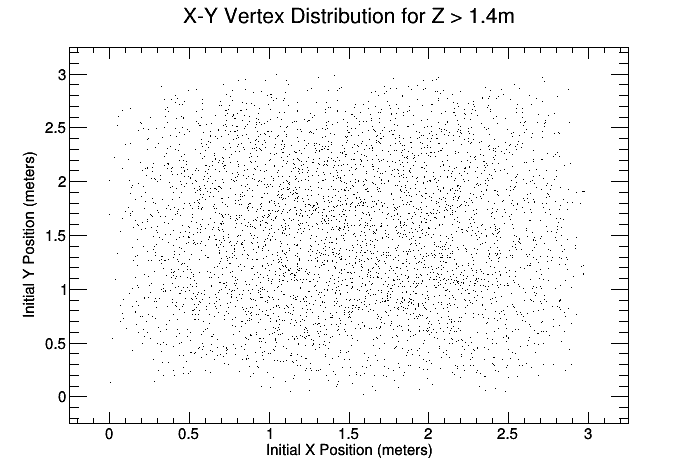
\includegraphics[width=0.6\textwidth]{NewANMReinSehgalImages/1-X-YVertexDistributionANMRS.png}
\caption{New $\bar{\nu}$-Mode Rein-Sehgal X-Y vertex distributions for muons that made it to the MRD and penetrated at least to the third layer of steel.}
\end{figure}

\begin{figure}[H]
\centering
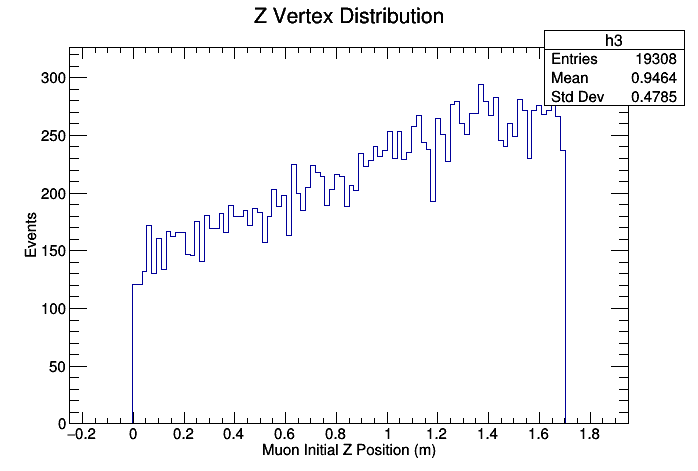
\includegraphics[width=0.6\textwidth]{NewANMReinSehgalImages/2-ZVertexDistributionANMRS.png}
\caption{New $\bar{\nu}$-Mode Rein-Sehgal Z vertex distributions for the interactions.}
\end{figure}

\begin{figure}[H]
\centering
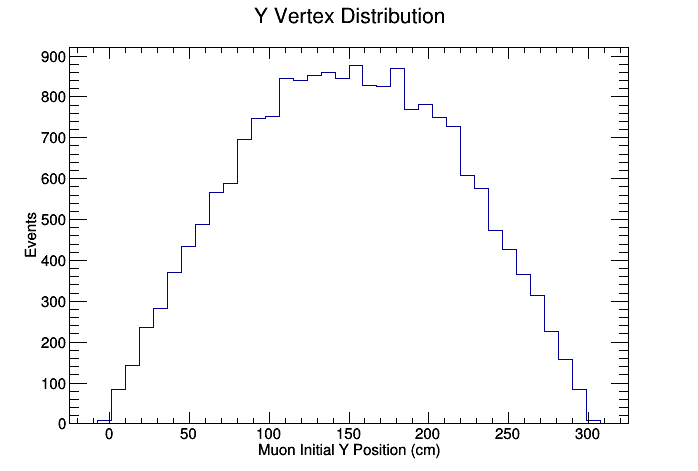
\includegraphics[width=0.6\textwidth]{NewANMReinSehgalImages/3-YVertexDistributionANMRS.png}
\caption{New $\bar{\nu}$-Mode Rein-Sehgal Y vertex distributions for the interactions.}
\end{figure}

\begin{figure}[H]
\centering
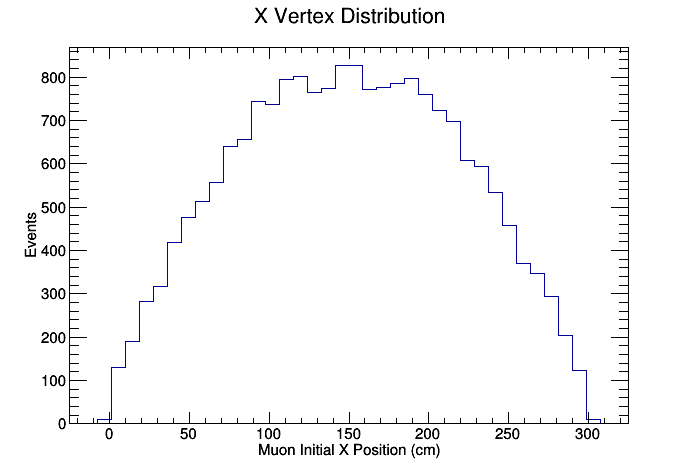
\includegraphics[width=0.6\textwidth]{NewANMReinSehgalImages/4-XVertexDistributionANMRS.png}
\caption{New $\bar{\nu}$-Mode Rein-Sehgal X vertex distributions for the interactions.}
\end{figure}

\begin{figure}[H]
\centering
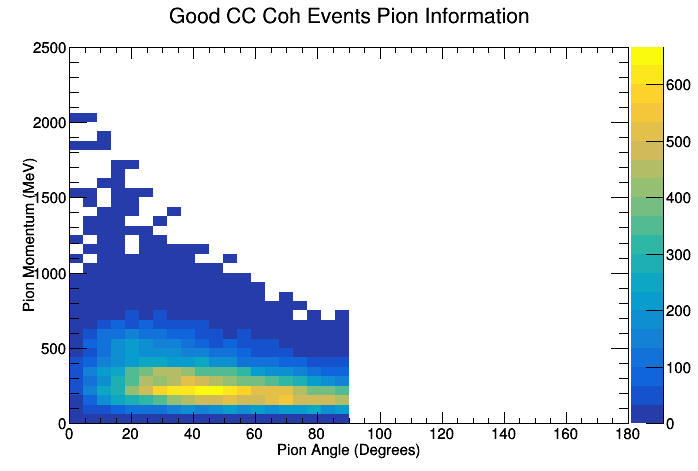
\includegraphics[width=0.6\textwidth]{NewANMReinSehgalImages/5-GoodCCCohPionInfoANMRS.png}
\caption{This is a 2D histogram for the momentum and angle of the pion in the CC Coh Pion events that met the qualification of being "good".}
\end{figure}

\begin{figure}[H]
\centering
\includegraphics[width=0.6\textwidth]{NewANMReinSehgalImages/6-GoodCCCohMuonInfoANMRS.png}
\caption{This is a 2D histogram for the momentum and angle of the muon in the CC Coh Pion events that met the qualification of being "good".}
\end{figure}

\begin{figure}[H]
\centering
\includegraphics[width=0.6\textwidth]{NewANMReinSehgalImages/7-LayerPenetrationANMRS.png}
\caption{This histogram shows the amount of muons that embedded (or "Stopped") in a corresponding layer of steel in our simulation.}
\end{figure}

\begin{figure}[H]
\centering
\includegraphics[width=0.6\textwidth]{NewANMReinSehgalImages/8-TotalCCCohPionInfoANMRS.png}
\caption{This is a 2D histogram for the momentum and angle of the pion in the total CC Coh Pion events.}
\end{figure}

\begin{figure}[H]
\centering
\includegraphics[width=0.6\textwidth]{NewANMReinSehgalImages/9-TotalCCCohMuonInfoANMRS.png}
\caption{This is a 2D histogram for the momentum and angle of the muon in the total CC Coh Pion events.}
\end{figure}

The NewANMReinSehgal.C macro also calculates many different quantities for the generated simulation of the events and saves the information in histograms that are later called upon through the plotting macros (which are after all of the analysis macros). The first quantity that is calculated for the different vertexes is the momentum of both the muon and the pion, which are both calculated using the equations:

\begin{equation}
|\vec{p}_\mu| = \sqrt{P_{\mu_x}^2 + P_{\mu_y}^2 + P_{\mu_z}^2}
\end{equation}

\begin{equation}
|\vec{p}_\pi| = \sqrt{P_{\pi_x}^2 + P_{\pi_y}^2 + P_{\pi_z}^2}
\end{equation}

\noindent
The momentum is reported in units of $MeV/c$.

The next quantity that is calculated in the macro is the angle from the beam-direction for both the muon and the pion, which are labeled as either $\theta_\mu$, or $\theta_\pi$, respectively. The angle from the beam-direction is the same as the angle from the z-direction, and this angle is known as the azimuthal angle. The calculation of the azimuthal angle is slightly more involved than the simple calculation used for finding the magnitude of the momentum of the two particles, and is calculated using the equations:

\begin{equation}
\theta_\mu = tan^{-1}(\sqrt{P_{\mu_x}^2 + P_{\mu_y}^2}/{P_{\mu_z}})
\end{equation}

\begin{equation}
\theta_\pi = tan^{-1}(\sqrt{P_{\pi_x}^2 + P_{\pi_y}^2}/{P_{\pi_z}})
\end{equation}

\noindent
The angles are reported in units of $\degree$, and should run from $0\degree$ to $180\degree$. In the case of Charged-Current Coherent Pion Production, the angle should never be larger than $90\degree$.

The last two quantities that this analysis macro calculates are the two different types of four-momentum transfers specific to this interaction, which are $Q^2$ and $|t|$. The $Q^2$ corresponds to the four-momentum transfer from the neutrino and muon to the nucleus and pion, and is calculated using the equation:

\begin{equation}
Q^2 = |(P_{\nu_\mu} - P_\mu)^2|
\end{equation}

\noindent
This equation is the four-momentum notational form. The code follows the equation below in order to compute $Q^2$:

\begin{equation}
Q^2 = |(P_{\nu_{\mu,x}} - P_{\mu_x})^2 + (P_{\nu_{\mu,y}} - P_{\mu_y})^2 + (P_{\nu_{\mu,z}} - P_{\mu_z})^2 + (P_{\nu_{\mu,E}} - P_{\mu_E})^2|
\end{equation}

\noindent
$Q^2$ is reported in units of $(MeV/c)^2$.

The $|t|$ corresponds to the four-momentum transfer from the neutrino, muon, and pion to the nucleus, and is calculated using the equation:

\begin{equation}
|t| = |(Q - P_\pi)^2| = |(P_{\nu_\mu} - P_\mu - P_\pi)^2|
\end{equation}

\noindent
This equation is the four-momentum notational form. The code follows the equation below in order to compute $|t|$:

\begin{equation}
|t| = |(P_{\nu_{\mu,x}} - P_{\mu_x} - P_{\pi_x})^2 + (P_{\nu_{\mu,y}} - P_{\mu_y} - P_{\pi_y})^2 + (P_{\nu_{\mu,z}} - P_{\mu_z} - P_{\pi_z})^2 + (P_{\nu_{\mu,E}} - P_{\mu_E} - P_{\pi_E})^2|
\end{equation}

\noindent
$|t|$ is reported in units of $(MeV/c)^2$.

%-----------------------------------------------------------------------------------------------------------------|
\subsection{NewANMBergerSehgal.C}
This file is the macro that corresponds to the "NewANMBergerSehgal.h" file, which connects with this file: "SciBooNE\textunderscore numubar\textunderscore coh\textunderscore RooTrack\textunderscore NEW.root". This file performs the main analysis for this generated sample, and then organizes the information into many different histograms. The histograms are then written to a file titled "totalmuoninfoBSBar.root" inside the "ROOTFILES" directory. The "ROOTFILES" directory is included in the SciBooNE-MC repository (it is absolutely pertinent that this directory be located where the macro files are located due to how the calls of the combined data macros reference the now saved histograms).

\begin{figure}[H]
\centering
\includegraphics[width=0.6\textwidth]{NewANMBergerSehgalImages/1-X-YVertexDistributionANMBS.png}
\caption{New $\bar{\nu}$-Mode Berger-Sehgal X-Y vertex distributions for muons that made it to the MRD and penetrated at least to the third layer of steel.}
\end{figure}

\begin{figure}[H]
\centering
\includegraphics[width=0.6\textwidth]{NewANMBergerSehgalImages/2-ZVertexDistributionANMBS.png}
\caption{New $\bar{\nu}$-Mode Berger-Sehgal Z vertex distributions for the interactions.}
\end{figure}

\begin{figure}[H]
\centering
\includegraphics[width=0.6\textwidth]{NewANMBergerSehgalImages/3-YVertexDistributionANMBS.png}
\caption{New $\bar{\nu}$-Mode Berger-Sehgal Y vertex distributions for the interactions.}
\end{figure}

\begin{figure}[H]
\centering
\includegraphics[width=0.6\textwidth]{NewANMBergerSehgalImages/4-XVertexDistributionANMBS.png}
\caption{New $\bar{\nu}$-Mode Berger-Sehgal X vertex distributions for the interactions.}
\end{figure}

\begin{figure}[H]
\centering
\includegraphics[width=0.6\textwidth]{NewANMBergerSehgalImages/5-GoodCCCohPionInfoANMBS.png}
\caption{This is a 2D histogram for the momentum and angle of the pion in the CC Coh Pion events that met the qualification of being "good".}
\end{figure}

\begin{figure}[H]
\centering
\includegraphics[width=0.6\textwidth]{NewANMBergerSehgalImages/6-GoodCCCohMuonInfoANMBS.png}
\caption{This is a 2D histogram for the momentum and angle of the muon in the CC Coh Pion events that met the qualification of being "good".}
\end{figure}

\begin{figure}[H]
\centering
\includegraphics[width=0.6\textwidth]{NewANMBergerSehgalImages/7-LayerPenetrationANMBS.png}
\caption{This histogram shows the amount of muons that embedded (or "Stopped") in a corresponding layer of steel in our simulation.}
\end{figure}

\begin{figure}[H]
\centering
\includegraphics[width=0.6\textwidth]{NewANMBergerSehgalImages/8-TotalCCCohPionInfoANMBS.png}
\caption{This is a 2D histogram for the momentum and angle of the pion in the total CC Coh Pion events.}
\end{figure}

\begin{figure}[H]
\centering
\includegraphics[width=0.6\textwidth]{NewANMBergerSehgalImages/9-TotalCCCohMuonInfoANMBS.png}
\caption{This is a 2D histogram for the momentum and angle of the muon in the total CC Coh Pion events.}
\end{figure}

The NewANMBergerSehgal.C macro also calculates many different quantities for the generated simulation of the events and saves the information in histograms that are later called upon through the plotting macros (which are after all of the analysis macros). The first quantity that is calculated for the different vertexes is the momentum of both the muon and the pion, which are both calculated using the equations:

\begin{equation}
|\vec{p}_\mu| = \sqrt{P_{\mu_x}^2 + P_{\mu_y}^2 + P_{\mu_z}^2}
\end{equation}

\begin{equation}
|\vec{p}_\pi| = \sqrt{P_{\pi_x}^2 + P_{\pi_y}^2 + P_{\pi_z}^2}
\end{equation}

\noindent
The momentum is reported in units of $MeV/c$.

The next quantity that is calculated in the macro is the angle from the beam-direction for both the muon and the pion, which are labeled as either $\theta_\mu$, or $\theta_\pi$, respectively. The angle from the beam-direction is the same as the angle from the z-direction, and this angle is known as the azimuthal angle. The calculation of the azimuthal angle is slightly more involved than the simple calculation used for finding the magnitude of the momentum of the two particles, and is calculated using the equations:

\begin{equation}
\theta_\mu = tan^{-1}(\sqrt{P_{\mu_x}^2 + P_{\mu_y}^2}/{P_{\mu_z}})
\end{equation}

\begin{equation}
\theta_\pi = tan^{-1}(\sqrt{P_{\pi_x}^2 + P_{\pi_y}^2}/{P_{\pi_z}})
\end{equation}

\noindent
The angles are reported in units of $\degree$, and should run from $0\degree$ to $180\degree$. In the case of Charged-Current Coherent Pion Production, the angle should never be larger than $90\degree$.

The last two quantities that this analysis macro calculates are the two different types of four-momentum transfers specific to this interaction, which are $Q^2$ and $|t|$. The $Q^2$ corresponds to the four-momentum transfer from the neutrino and muon to the nucleus and pion, and is calculated using the equation:

\begin{equation}
Q^2 = |(P_{\nu_\mu} - P_\mu)^2|
\end{equation}

\noindent
This equation is the four-momentum notational form. The code follows the equation below in order to compute $Q^2$:

\begin{equation}
Q^2 = |(P_{\nu_{\mu,x}} - P_{\mu_x})^2 + (P_{\nu_{\mu,y}} - P_{\mu_y})^2 + (P_{\nu_{\mu,z}} - P_{\mu_z})^2 + (P_{\nu_{\mu,E}} - P_{\mu_E})^2|
\end{equation}

\noindent
$Q^2$ is reported in units of $(MeV/c)^2$.

The $|t|$ corresponds to the four-momentum transfer from the neutrino, muon, and pion to the nucleus, and is calculated using the equation:

\begin{equation}
|t| = |(Q - P_\pi)^2| = |(P_{\nu_\mu} - P_\mu - P_\pi)^2|
\end{equation}

\noindent
This equation is the four-momentum notational form. The code follows the equation below in order to compute $|t|$:

\begin{equation}
|t| = |(P_{\nu_{\mu,x}} - P_{\mu_x} - P_{\pi_x})^2 + (P_{\nu_{\mu,y}} - P_{\mu_y} - P_{\pi_y})^2 + (P_{\nu_{\mu,z}} - P_{\mu_z} - P_{\pi_z})^2 + (P_{\nu_{\mu,E}} - P_{\mu_E} - P_{\pi_E})^2|
\end{equation}

\noindent
$|t|$ is reported in units of $(MeV/c)^2$.

%-----------------------------------------------------------------------------------------------------------------|
\subsection{NMCombinedPlots.C}
I need to come back and insert all of my images here.

\begin{figure}[H]
\centering
\includegraphics[width=0.6\textwidth]{NMCombinedPlotsImages/1-NMCombinedPlots.png}
\caption{}
\end{figure}

\begin{figure}[H]
\centering
\includegraphics[width=0.6\textwidth]{NMCombinedPlotsImages/2-NMCombinedPlots.png}
\caption{}
\end{figure}

\begin{figure}[H]
\centering
\includegraphics[width=0.6\textwidth]{NMCombinedPlotsImages/3-NMCombinedPlots.png}
\caption{}
\end{figure}

\begin{figure}[H]
\centering
\includegraphics[width=0.6\textwidth]{NMCombinedPlotsImages/4-NMCombinedPlots.png}
\caption{}
\end{figure}

\begin{figure}[H]
\centering
\includegraphics[width=0.6\textwidth]{NMCombinedPlotsImages/5-NMCombinedPlots.png}
\caption{}
\end{figure}

\begin{figure}[H]
\centering
\includegraphics[width=0.6\textwidth]{NMCombinedPlotsImages/6-NMCombinedPlots.png}
\caption{}
\end{figure}

\begin{figure}[H]
\centering
\includegraphics[width=0.6\textwidth]{NMCombinedPlotsImages/7-NMCombinedPlots.png}
\caption{}
\end{figure}

\begin{figure}[H]
\centering
\includegraphics[width=0.6\textwidth]{NMCombinedPlotsImages/8-NMCombinedPlots.png}
\caption{}
\end{figure}

\begin{figure}[H]
\centering
\includegraphics[width=0.6\textwidth]{NMCombinedPlotsImages/9-NMCombinedPlots.png}
\caption{}
\end{figure}

\begin{figure}[H]
\centering
\includegraphics[width=0.6\textwidth]{NMCombinedPlotsImages/10-NMCombinedPlots.png}
\caption{}
\end{figure}

\begin{figure}[H]
\centering
\includegraphics[width=0.6\textwidth]{NMCombinedPlotsImages/11-NMCombinedPlots.png}
\caption{}
\end{figure}

\begin{figure}[H]
\centering
\includegraphics[width=0.6\textwidth]{NMCombinedPlotsImages/12-NMCombinedPlots.png}
\caption{}
\end{figure}

\begin{figure}[H]
\centering
\includegraphics[width=0.6\textwidth]{NMCombinedPlotsImages/13-NMCombinedPlots.png}
\caption{}
\end{figure}

\begin{figure}[H]
\centering
\includegraphics[width=0.6\textwidth]{NMCombinedPlotsImages/14-NMCombinedPlots.png}
\caption{}
\end{figure}

\begin{figure}[H]
\centering
\includegraphics[width=0.6\textwidth]{NMCombinedPlotsImages/15-NMCombinedPlots.png}
\caption{}
\end{figure}

\begin{figure}[H]
\centering
\includegraphics[width=0.6\textwidth]{NMCombinedPlotsImages/16-NMCombinedPlots.png}
\caption{}
\end{figure}

\begin{figure}[H]
\centering
\includegraphics[width=0.6\textwidth]{NMCombinedPlotsImages/17-NMCombinedPlots.png}
\caption{}
\end{figure}

\begin{figure}[H]
\centering
\includegraphics[width=0.6\textwidth]{NMCombinedPlotsImages/18-NMCombinedPlots.png}
\caption{}
\end{figure}

\begin{figure}[H]
\centering
\includegraphics[width=0.6\textwidth]{NMCombinedPlotsImages/19-NMCombinedPlots.png}
\caption{}
\end{figure}

\begin{figure}[H]
\centering
\includegraphics[width=0.6\textwidth]{NMCombinedPlotsImages/20-NMCombinedPlots.png}
\caption{}
\end{figure}

\begin{figure}[H]
\centering
\includegraphics[width=0.6\textwidth]{NMCombinedPlotsImages/21-NMCombinedPlots.png}
\caption{}
\end{figure}

\begin{figure}[H]
\centering
\includegraphics[width=0.6\textwidth]{NMCombinedPlotsImages/22-NMCombinedPlots.png}
\caption{}
\end{figure}

\begin{figure}[H]
\centering
\includegraphics[width=0.6\textwidth]{NMCombinedPlotsImages/23-NMCombinedPlots.png}
\caption{}
\end{figure}

\begin{figure}[H]
\centering
\includegraphics[width=0.6\textwidth]{NMCombinedPlotsImages/24-NMCombinedPlots.png}
\caption{}
\end{figure}

\begin{figure}[H]
\centering
\includegraphics[width=0.6\textwidth]{NMCombinedPlotsImages/25-NMCombinedPlots.png}
\caption{}
\end{figure}

%-----------------------------------------------------------------------------------------------------------------|
\subsection{NMPionPlotting.C}
I need to come back and insert all of my images here.

\begin{figure}[H]
\centering
\includegraphics[width=0.6\textwidth]{NMPionPlottingImages/1-NMPionPlotting.png}
\caption{}
\end{figure}

\begin{figure}[H]
\centering
\includegraphics[width=0.6\textwidth]{NMPionPlottingImages/2-NMPionPlotting.png}
\caption{}
\end{figure}

\begin{figure}[H]
\centering
\includegraphics[width=0.6\textwidth]{NMPionPlottingImages/3-NMPionPlotting.png}
\caption{}
\end{figure}

\begin{figure}[H]
\centering
\includegraphics[width=0.6\textwidth]{NMPionPlottingImages/4-NMPionPlotting.png}
\caption{}
\end{figure}

\begin{figure}[H]
\centering
\includegraphics[width=0.6\textwidth]{NMPionPlottingImages/5-NMPionPlotting.png}
\caption{}
\end{figure}

\begin{figure}[H]
\centering
\includegraphics[width=0.6\textwidth]{NMPionPlottingImages/6-NMPionPlotting.png}
\caption{}
\end{figure}

\begin{figure}[H]
\centering
\includegraphics[width=0.6\textwidth]{NMPionPlottingImages/7-NMPionPlotting.png}
\caption{}
\end{figure}

\begin{figure}[H]
\centering
\includegraphics[width=0.6\textwidth]{NMPionPlottingImages/8-NMPionPlotting.png}
\caption{}
\end{figure}

\begin{figure}[H]
\centering
\includegraphics[width=0.6\textwidth]{NMPionPlottingImages/9-NMPionPlotting.png}
\caption{}
\end{figure}

\begin{figure}[H]
\centering
\includegraphics[width=0.6\textwidth]{NMPionPlottingImages/10-NMPionPlotting.png}
\caption{}
\end{figure}

\begin{figure}[H]
\centering
\includegraphics[width=0.6\textwidth]{NMPionPlottingImages/11-NMPionPlotting.png}
\caption{}
\end{figure}

\begin{figure}[H]
\centering
\includegraphics[width=0.6\textwidth]{NMPionPlottingImages/12-NMPionPlotting.png}
\caption{}
\end{figure}

%-----------------------------------------------------------------------------------------------------------------|
\subsection{NMFourSquaredPlotting.C}
I need to come back and insert all of my images here.

\begin{figure}[H]
\centering
\includegraphics[width=0.6\textwidth]{NMFourSquaredPlottingImages/1-NMFourSquaredPlotting.png}
\caption{}
\end{figure}

\begin{figure}[H]
\centering
\includegraphics[width=0.6\textwidth]{NMFourSquaredPlottingImages/2-NMFourSquaredPlotting.png}
\caption{}
\end{figure}

\begin{figure}[H]
\centering
\includegraphics[width=0.6\textwidth]{NMFourSquaredPlottingImages/3-NMFourSquaredPlotting.png}
\caption{}
\end{figure}

\begin{figure}[H]
\centering
\includegraphics[width=0.6\textwidth]{NMFourSquaredPlottingImages/4-NMFourSquaredPlotting.png}
\caption{}
\end{figure}

\begin{figure}[H]
\centering
\includegraphics[width=0.6\textwidth]{NMFourSquaredPlottingImages/5-NMFourSquaredPlotting.png}
\caption{}
\end{figure}

\begin{figure}[H]
\centering
\includegraphics[width=0.6\textwidth]{NMFourSquaredPlottingImages/6-NMFourSquaredPlotting.png}
\caption{}
\end{figure}

%-----------------------------------------------------------------------------------------------------------------|
\subsection{ANMCombinedPlots.C}
I need to come back and insert all of my images here.

\begin{figure}[H]
\centering
\includegraphics[width=0.6\textwidth]{ANMCombinedPlotsImages/1-ANMCombinedPlots.png}
\caption{}
\end{figure}

\begin{figure}[H]
\centering
\includegraphics[width=0.6\textwidth]{ANMCombinedPlotsImages/2-ANMCombinedPlots.png}
\caption{}
\end{figure}

\begin{figure}[H]
\centering
\includegraphics[width=0.6\textwidth]{ANMCombinedPlotsImages/3-ANMCombinedPlots.png}
\caption{}
\end{figure}

\begin{figure}[H]
\centering
\includegraphics[width=0.6\textwidth]{ANMCombinedPlotsImages/4-ANMCombinedPlots.png}
\caption{}
\end{figure}

\begin{figure}[H]
\centering
\includegraphics[width=0.6\textwidth]{ANMCombinedPlotsImages/5-ANMCombinedPlots.png}
\caption{}
\end{figure}

\begin{figure}[H]
\centering
\includegraphics[width=0.6\textwidth]{ANMCombinedPlotsImages/6-ANMCombinedPlots.png}
\caption{}
\end{figure}

\begin{figure}[H]
\centering
\includegraphics[width=0.6\textwidth]{ANMCombinedPlotsImages/7-ANMCombinedPlots.png}
\caption{}
\end{figure}

\begin{figure}[H]
\centering
\includegraphics[width=0.6\textwidth]{ANMCombinedPlotsImages/8-ANMCombinedPlots.png}
\caption{}
\end{figure}

\begin{figure}[H]
\centering
\includegraphics[width=0.6\textwidth]{ANMCombinedPlotsImages/9-ANMCombinedPlots.png}
\caption{}
\end{figure}

\begin{figure}[H]
\centering
\includegraphics[width=0.6\textwidth]{ANMCombinedPlotsImages/10-ANMCombinedPlots.png}
\caption{}
\end{figure}

\begin{figure}[H]
\centering
\includegraphics[width=0.6\textwidth]{ANMCombinedPlotsImages/11-ANMCombinedPlots.png}
\caption{}
\end{figure}

\begin{figure}[H]
\centering
\includegraphics[width=0.6\textwidth]{ANMCombinedPlotsImages/12-ANMCombinedPlots.png}
\caption{}
\end{figure}

\begin{figure}[H]
\centering
\includegraphics[width=0.6\textwidth]{ANMCombinedPlotsImages/13-ANMCombinedPlots.png}
\caption{}
\end{figure}

\begin{figure}[H]
\centering
\includegraphics[width=0.6\textwidth]{ANMCombinedPlotsImages/14-ANMCombinedPlots.png}
\caption{}
\end{figure}

\begin{figure}[H]
\centering
\includegraphics[width=0.6\textwidth]{ANMCombinedPlotsImages/15-ANMCombinedPlots.png}
\caption{}
\end{figure}

\begin{figure}[H]
\centering
\includegraphics[width=0.6\textwidth]{ANMCombinedPlotsImages/16-ANMCombinedPlots.png}
\caption{}
\end{figure}

\begin{figure}[H]
\centering
\includegraphics[width=0.6\textwidth]{ANMCombinedPlotsImages/17-ANMCombinedPlots.png}
\caption{}
\end{figure}

\begin{figure}[H]
\centering
\includegraphics[width=0.6\textwidth]{ANMCombinedPlotsImages/18-ANMCombinedPlots.png}
\caption{}
\end{figure}

%-----------------------------------------------------------------------------------------------------------------|
\subsection{ANMPionPlotting.C}
I need to come back and insert all of my images here.

\begin{figure}[H]
\centering
\includegraphics[width=0.6\textwidth]{ANMPionPlottingImages/1-ANMPionPlotting.png}
\caption{}
\end{figure}

\begin{figure}[H]
\centering
\includegraphics[width=0.6\textwidth]{ANMPionPlottingImages/2-ANMPionPlotting.png}
\caption{}
\end{figure}

\begin{figure}[H]
\centering
\includegraphics[width=0.6\textwidth]{ANMPionPlottingImages/3-ANMPionPlotting.png}
\caption{}
\end{figure}

\begin{figure}[H]
\centering
\includegraphics[width=0.6\textwidth]{ANMPionPlottingImages/4-ANMPionPlotting.png}
\caption{}
\end{figure}

\begin{figure}[H]
\centering
\includegraphics[width=0.6\textwidth]{ANMPionPlottingImages/5-ANMPionPlotting.png}
\caption{}
\end{figure}

\begin{figure}[H]
\centering
\includegraphics[width=0.6\textwidth]{ANMPionPlottingImages/6-ANMPionPlotting.png}
\caption{}
\end{figure}

\begin{figure}[H]
\centering
\includegraphics[width=0.6\textwidth]{ANMPionPlottingImages/7-ANMPionPlotting.png}
\caption{}
\end{figure}

\begin{figure}[H]
\centering
\includegraphics[width=0.6\textwidth]{ANMPionPlottingImages/8-ANMPionPlotting.png}
\caption{}
\end{figure}

\begin{figure}[H]
\centering
\includegraphics[width=0.6\textwidth]{ANMPionPlottingImages/9-ANMPionPlotting.png}
\caption{}
\end{figure}

\begin{figure}[H]
\centering
\includegraphics[width=0.6\textwidth]{ANMPionPlottingImages/10-ANMPionPlotting.png}
\caption{}
\end{figure}

\begin{figure}[H]
\centering
\includegraphics[width=0.6\textwidth]{ANMPionPlottingImages/11-ANMPionPlotting.png}
\caption{}
\end{figure}

\begin{figure}[H]
\centering
\includegraphics[width=0.6\textwidth]{ANMPionPlottingImages/12-ANMPionPlotting.png}
\caption{}
\end{figure}

%-----------------------------------------------------------------------------------------------------------------|
\subsection{ANMFourSquaredPlotting.C}
I need to come back and insert all of my images here.

\begin{figure}[H]
\centering
\includegraphics[width=0.6\textwidth]{ANMFourSquaredPlottingImages/1-ANMFourSquaredPlotting.png}
\caption{}
\end{figure}

\begin{figure}[H]
\centering
\includegraphics[width=0.6\textwidth]{ANMFourSquaredPlottingImages/2-ANMFourSquaredPlotting.png}
\caption{}
\end{figure}

\begin{figure}[H]
\centering
\includegraphics[width=0.6\textwidth]{ANMFourSquaredPlottingImages/3-ANMFourSquaredPlotting.png}
\caption{}
\end{figure}

\begin{figure}[H]
\centering
\includegraphics[width=0.6\textwidth]{ANMFourSquaredPlottingImages/4-ANMFourSquaredPlotting.png}
\caption{}
\end{figure}

\begin{figure}[H]
\centering
\includegraphics[width=0.6\textwidth]{ANMFourSquaredPlottingImages/5-ANMFourSquaredPlotting.png}
\caption{}
\end{figure}

\begin{figure}[H]
\centering
\includegraphics[width=0.6\textwidth]{ANMFourSquaredPlottingImages/6-ANMFourSquaredPlotting.png}
\caption{}
\end{figure}
%%%%%%%%%%%%%%%%%%%%%%%%%%%%%%%% The Files and Their Outputs section ends here! %%%%%%%%%%%%%%%%%%%%%%%%%%%%%%%%%|



%======================================== A New Section Begins Here =============================================|
\section{Steps for Running the Code}
The instructions on how to run the code and the order the files need to run in so that there are no resulting error messages, or other issues while running the code, are detailed in this section.

\begin{adjustwidth}{4.0em}{0pt}
\begin{steps}
  \item This is the first step. (Run the NewNM macros and the NewANM macros and the OldNM macro.)
  \item This is the second step. (Run the combined plotting macros.)
  \item This is the third step. (Run the Pion Plotting macros.)
  \item Etc. (Run the FourSquaredMomentum macros.)
\end{steps}
\end{adjustwidth}
%%%%%%%%%%%%%%%%%%%%%%%%%%%%%% The Steps for Running the Code section ends here! %%%%%%%%%%%%%%%%%%%%%%%%%%%%%%%|



%===================================== A New Section Begins Here ===============================================|
\section{Closing Remarks and Cautions}
These are just a few cautionary suggestions for potential issues that might be encountered while trying to use this code. This will also be where and further closing remarks can be made.
%%%%%%%%%%%%%%%%%%%%%%%%%%%%% The Steps for Running the Code section ends here! %%%%%%%%%%%%%%%%%%%%%%%%%%%%%%%%|



%====================================== A New Section Begins Here ==============================================|
\section{Acknowledgements}
Thank everyone who helped, and thank everyone who gave their inputs into your acceptance study. YOU NEED TO GIVE A HUGE AND SPECIAL THANKS TO DR. ASAADI RIGHT HERE! (He has been suuuuuuuper patient...)
%%%%%%%%%%%%%%%%%%%%%%%%%%%%%%%%% The Acknowledgements section ends here! %%%%%%%%%%%%%%%%%%%%%%%%%%%%%%%%%%%%%%|



%===================================== A New Section Begins Here ===============================================|
\section{Figures and Tables} \label{sec:FigTab}
\subsection{List of Figures}
There will eventually be a huge list of figures here.

\subsection{List of Tables}
There will eventually be the event reduction tables and 2D histogram tables here.

\newpage
\begin{landscape}
\begin{table}
\centering
\caption{Table for 2D Histogram for New NM-Rein-Sehgal}
\begin{adjustbox}{width=\paperwidth}
\csvautotabular{TechNoteTables/New-NM-RS.csv}
\end{adjustbox}
\end{table}
\end{landscape}

\newpage
\begin{landscape}
\begin{table}
\centering
\caption{Table for 2D Histogram for New NM-Berger-Sehgal}
\begin{adjustbox}{width=\paperwidth}
\csvautotabular{TechNoteTables/New-NM-BS.csv}
\end{adjustbox}
\end{table}
\end{landscape}

\newpage
\begin{landscape}
\begin{table}
\centering
\caption{Table for 2D Histogram for Old NM-Rein-Sehgal}
\begin{adjustbox}{width=\paperwidth}
\csvautotabular{TechNoteTables/Old-NM-RS.csv}
\end{adjustbox}
\end{table}
\end{landscape}

\newpage
\begin{landscape}
\begin{table}
\centering
\caption{Table for 2D Histogram for New ANM-Rein-Sehgal}
\begin{adjustbox}{width=\paperwidth}
\csvautotabular{TechNoteTables/New-ANM-RS.csv}
\end{adjustbox}
\end{table}
\end{landscape}

\newpage
\begin{landscape}
\begin{table}
\centering
\caption{Table for 2D Histogram for New ANM-Berger-Sehgal}
\begin{adjustbox}{width=\paperwidth}
\csvautotabular{TechNoteTables/New-ANM-BS.csv}
\end{adjustbox}
\end{table}
\end{landscape}
%%%%%%%%%%%%%%%%%%%%%%%%%%%%%%%%%%%%%%%%%%% The Appendix section ends here! %%%%%%%%%%%%%%%%%%%%%%%%%%%%%%%%%%%%|



\end{document}
%|------------------------------The Document Ends Here----------------------------------|